% ============================================================
% Chapter: Wilkinson Power Divider, Mixer, and LO Buffer
% Converted from Thesis.docx
%
% NOTE TO TEAM: This file assumes the following packages are loaded
% in the main thesis preamble:
%   \usepackage{graphicx}
%   \usepackage{amsmath}
%   \usepackage{amssymb}
%   \usepackage{booktabs}
%   \usepackage{siunitx}      % for \si{} units, optional
%   \usepackage{hyperref}     % for \ref / \label cross-referencing
% Adjust \graphicspath below to point at the figures/ folder, or
% move the figures/ folder into your main Overleaf project and
% update the path accordingly.
% ============================================================

\graphicspath{{figures/}}

\chapter{Power Divider}

\section{Wilkinson Power Divider}

\subsection{Introduction}

Power dividers are essential passive components in radio frequency (RF) and microwave systems, used to split an input signal into two or more output signals with specific amplitude and phase characteristics. They are commonly employed in applications such as phased-array antennas, signal distribution networks, balanced mixers, and measurement systems.

In their basic form, RF power dividers are designed to split the input power equally among the output ports (e.g., a 3~dB power divider splits the input power equally into two ports), although unequal (asymmetric) division is also possible depending on the design. Ideal power dividers are expected to exhibit characteristics such as minimal insertion loss, good impedance matching at all ports, and high isolation between output ports.

Real-world power dividers are typically implemented using transmission lines or lumped-element networks, and they come in several types, including resistive dividers, Wilkinson power dividers, and hybrid couplers. Each type has trade-offs in terms of bandwidth, loss, isolation, and size, making the selection application-dependent.

\subsection{Literature Review}

\subsubsection{Performance Metrics}

\paragraph{Insertion Loss}

Insertion loss is a key performance metric for power dividers, representing the amount of signal power lost as it passes through the device. It quantifies how much lower the output power is, compared to the input. In an ideal power divider, the insertion loss is only due to power division. For example, a 2-way equal power divider ideally introduces a 3~dB loss, meaning each output receives half the input power:
\begin{equation}
\text{Insertion loss} = 10\log N, \quad N: \text{number of output ports}
\end{equation}
\begin{equation}
\text{For 2 outports} \rightarrow IL = 10\log 2 = 3~\text{dB}
\end{equation}

In practical implementations, the total insertion loss is greater than the theoretical value, due to:
\begin{itemize}
    \item Resistive losses in conductors and isolation resistors.
    \item Dielectric losses in the substrate material.
    \item Mismatches between ports, leading to partial reflections.
    \item Radiation losses, especially at higher frequencies or in open structures.
\end{itemize}

\paragraph{I/O Matching}

I/O matching refers to the process of ensuring that the input and output ports of a power divider (or any RF component) are impedance-matched to the system characteristic impedance (typically 50~$\Omega$). Proper matching is essential to maximize power transfer and minimize reflections.

In our work the input matching is for 30~$\Omega$ while the output is for 50~$\Omega$.

\paragraph{Isolation}

Isolation refers to how well two output ports of a power divider are electrically separated from each other. In other words, it measures how much signal leaks from one output port to another, which ideally should be zero.
\begin{equation}
\text{Isolation} = -20\log\left(|S_{23}|\right)
\end{equation}

\paragraph{Magnitude Imbalance}

Magnitude imbalance refers to the difference in output signal amplitudes between two (or more) output ports of a power divider. Ideally, a power divider distributes power equally, but in practical implementations, small differences occur due to component tolerances, layout asymmetries, or frequency-dependent effects.
\begin{equation}
\text{Magnitude imbalance (dB)} = 20\log\left(\frac{V_2}{V_1}\right)
\end{equation}
where $V_1, V_2$ are the output voltage magnitudes (or equivalently, power levels). If both outputs are equal, the magnitude imbalance is 0~dB.

\paragraph{Phase Imbalance}

Phase imbalance refers to the difference in phase between the output signals of a power divider. Ideally, in a symmetric 2-way power divider, both outputs should have the same phase or a specific known phase difference (e.g., $90^\circ$ in quadrature hybrids). Any deviation from this expected phase difference is defined as phase imbalance. For a 2-way equal-split power divider (expecting equal phase):
\begin{equation}
\text{Phase imbalance (degree)} = \angle V_2 - \angle V_1
\end{equation}
where $\angle V_1, \angle V_2$ are the phases of the output signals.

\paragraph{Linearity}

Power dividers are expected to operate as passive, linear components, meaning they should not distort the input signal or generate unwanted spectral components. In practice, their linearity refers to how well they maintain signal integrity across a range of input power levels, without introducing non-linear behavior such as harmonic or intermodulation distortion.

\subsubsection{Types of Power Dividers}

Power dividers and combiners are implemented using diverse topologies, each offering specific trade-offs across key performance metrics such as bandwidth, isolation, insertion loss, and impedance matching to suit particular application requirements. These circuits are generally classified into the following primary categories.

\paragraph{Resistive Power Divider}

Uses only resistors to divide power equally or unequally between ports.

\begin{figure}[htbp]
    \centering
    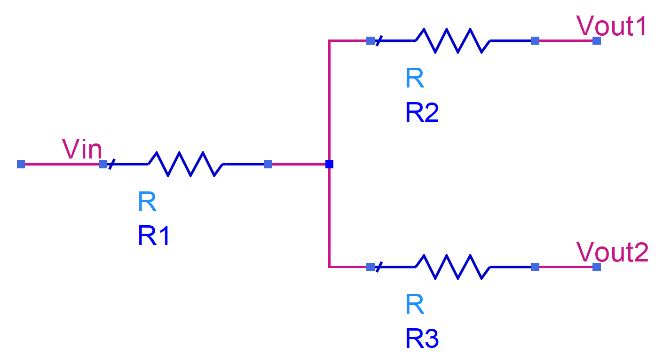
\includegraphics[width=0.6\textwidth]{thesis_chapter_latex/figures/fig_resistive_divider.png}
    \caption{Resistive power divider}
    \label{fig:resistive_divider}
\end{figure}

\textbf{Advantages} --- Demonstrates ultra-wideband operation, utilizes a compact and mathematically simple architecture, and exhibits no dependency on transmission line electrical length.

\textbf{Limitations} --- Suffers from a total lack of port-to-port isolation and introduces significant insertion loss (6~dB minimum for a symmetrical two-way split) due to inherent resistive dissipation.

\textbf{Applications} --- Primarily utilized in low-frequency networks, DC-to-RF wideband systems, and measurement/test instrument configurations where wide frequency coverage takes precedence over power efficiency.

\paragraph{Wilkinson Power Divider}

\textbf{Operation} --- Utilizes quarter-wave $\lambda/4$ impedance-transforming transmission lines alongside an integrated isolation resistor to achieve power division while simultaneously ensuring robust impedance matching across all ports.

\textbf{Key Features} --- Provides excellent port-to-port isolation and minimizes insertion loss by eliminating resistive dissipation under perfectly balanced, in-phase operating conditions.

\begin{figure}[htbp]
    \centering
    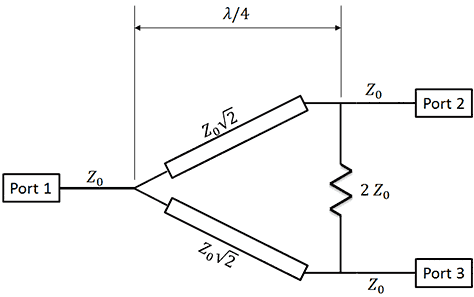
\includegraphics[width=0.55\textwidth]{thesis_chapter_latex/figures/fig_wilkinson_divider.png}
    \caption{Wilkinson power divider}
    \label{fig:wilkinson_divider}
\end{figure}

\textbf{Advantages} --- Achieves excellent, simultaneous impedance matching across all ports, provides high isolation between output ports, and exhibits minimal insertion loss, approaching the ideal theoretical limit of 3~dB for a symmetrical two-way split.

\textbf{Limitations} --- Inherently constrained to narrowband operation unless optimized via multi-section or tapered transmission line profiles; additionally, the layout demands a significantly larger physical footprint due to the required quarter-wave $\lambda/4$ line geometries.

\textbf{Applications} --- Primarily deployed in narrowband RF and microwave architectures, as well as corporate antenna feed networks where power efficiency and port isolation are critical design parameters.

\section{Design Methodology}

\subsection{Design Specifications}

\begin{table}[htbp]
    \centering
    \caption{Power divider design specifications}
    \label{tab:pd_design_specs}
    \begin{tabular}{ll}
        \toprule
        Parameter & Spec \\
        \midrule
        Insertion loss        & $<$ 7~dB \\
        I/O Return loss       & $<$ $-7$~dB \\
        Isolation             & $>$ 7~dB \\
        Magnitude imbalance   & $<$ 0.5~dB \\
        Phase imbalance       & $<$ 0.5 degree \\
        IIP3                  & $>$ 40~dBm \\
        \bottomrule
    \end{tabular}
\end{table}

\subsection{Topology Selection}

\textbf{Design Objectives and Scope} --- The specified topology must achieve ultra-wideband performance spanning from 400~MHz to 8~GHz. To satisfy this multi-octave bandwidth requirement, a wideband power divider architecture was selected based on established academic literature.

\textbf{Component Constraints} --- The inclusion of the lower frequency band (specifically from 400~MHz up to 2~GHz) poses a unique design challenge, as it necessitates relatively large integrated inductor values reaching up to 1.6~nH. Managing the physical layout and parasitic effects of these larger components represents a critical factor in maintaining performance across the entire band.

\textbf{Implementation Architecture} --- The specific schematic topology is detailed in Figure~\ref{fig:compact_divider_topology}. However, based on our optimization and bandwidth requirements, the implementation was scaled down to a two-stage network rather than the four-stage configuration illustrated in the original reference paper.

\begin{figure}[htbp]
    \centering
    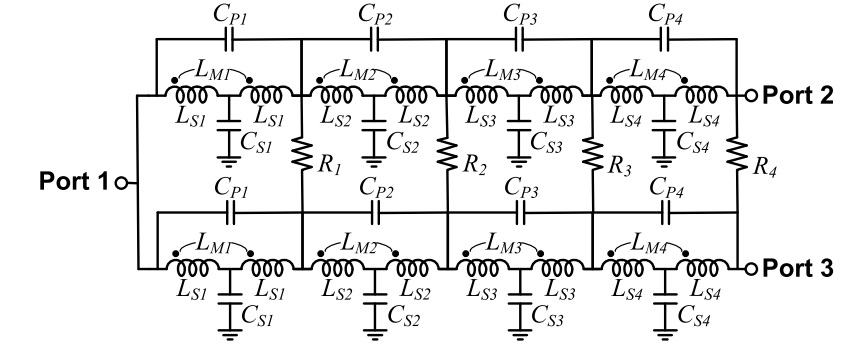
\includegraphics[width=\textwidth]{thesis_chapter_latex/figures/fig_compact_divider_topology.png}
    \caption{Super compact and ultrabroadband power divider topology}
    \label{fig:compact_divider_topology}
\end{figure}

\section{Power Divider Layout}

The layout routing is strictly engineered to enforce a highly symmetric design. This geometric symmetry is critical to ensuring balanced phase and amplitude distribution between the differential signal paths, minimizing phase imbalances and unwanted parasitic asymmetries.

To mitigate electromagnetic coupling and crosstalk, a dedicated ground shielding trace is routed directly between the differential paths. This physical isolation line acts as a localized shield, significantly improving path-to-path isolation and preserving signal integrity across the high-frequency operating band.

\begin{figure}[htbp]
    \centering
    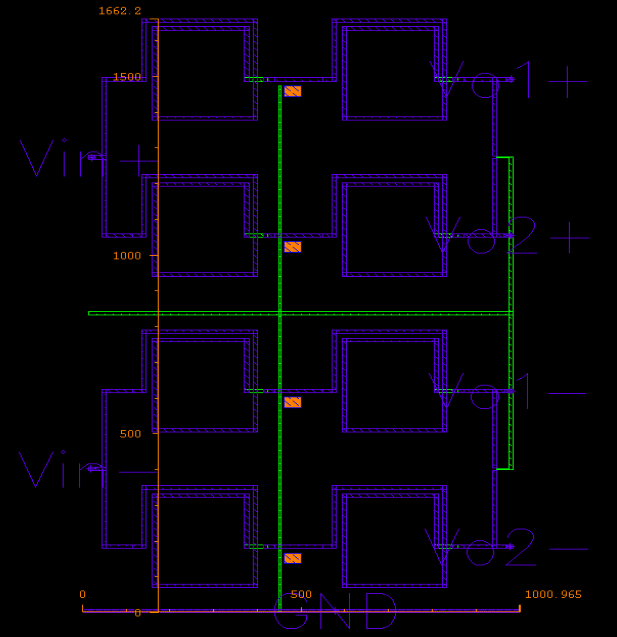
\includegraphics[width=0.6\textwidth]{thesis_chapter_latex/figures/fig_power_divider_layout.png}
    \caption{Power divider layout}
    \label{fig:power_divider_layout}
\end{figure}

\begin{equation}
\text{Area} = 1.000965 \times 1.6622 = 1.6638~\text{mm}^2
\end{equation}

The final layout occupies a significantly large physical area. This expanded footprint is directly driven by the large-value integrated inductors required to fulfill the performance specifications at the lower end of the operating band, specifically from 400~MHz to 2~GHz.

\section{Post-Layout Simulation Results for Power Divider}

\begin{figure}[htbp]
    \centering
    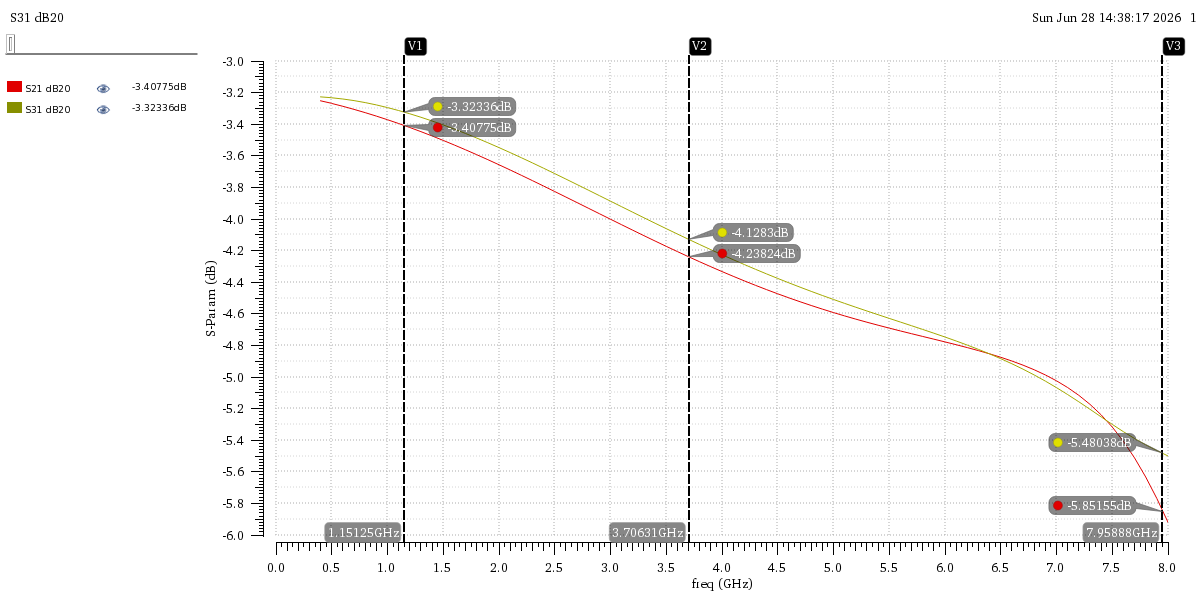
\includegraphics[width=\textwidth]{thesis_chapter_latex/figures/fig_power_divider_il_nominal.png}
    \caption{Power divider insertion loss for 2 paths at nominal case}
    \label{fig:pd_il_nominal}
\end{figure}

\subsection{Insertion Loss}

\textbf{Insertion Loss Analysis} --- As illustrated in Figure~\ref{fig:pd_il_nominal}, the insertion loss profiles of both paths track closely across the band, exhibiting minor divergence only at the upper frequency limit. Crucially, the total insertion loss remains below 6~dB across the entire operating range, successfully satisfying the design specification of 7~dB.

\begin{figure}[htbp]
    \centering
    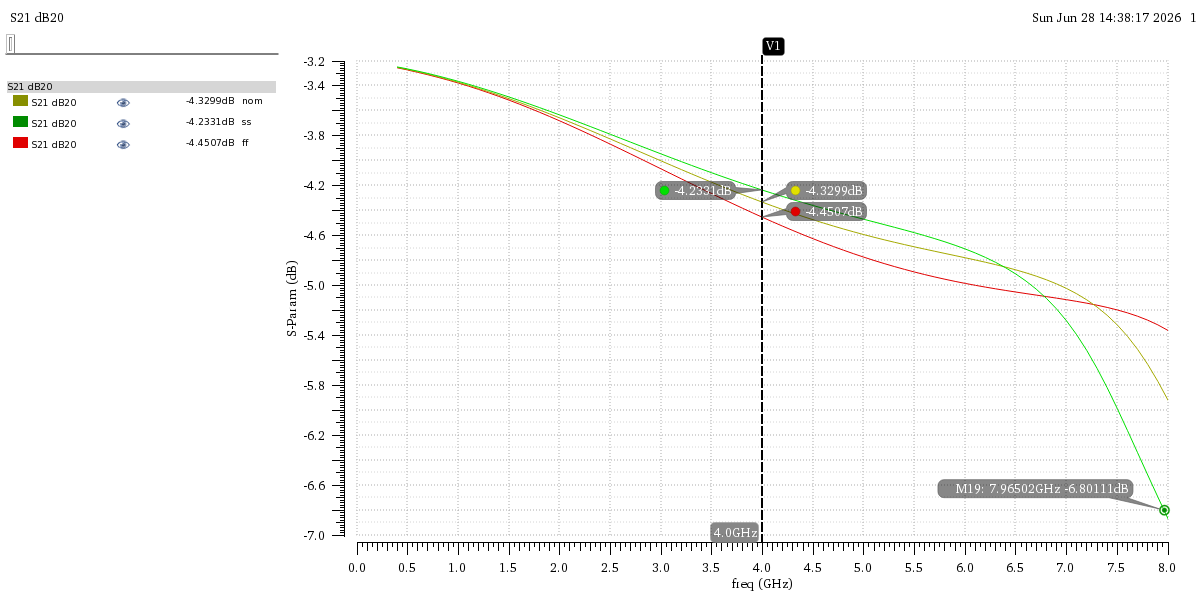
\includegraphics[width=\textwidth]{thesis_chapter_latex/figures/fig_power_divider_il_path1_corners.png}
    \caption{Power divider insertion loss, Path 1, across corners}
    \label{fig:pd_il_path1_corners}
\end{figure}

\begin{figure}[htbp]
    \centering
    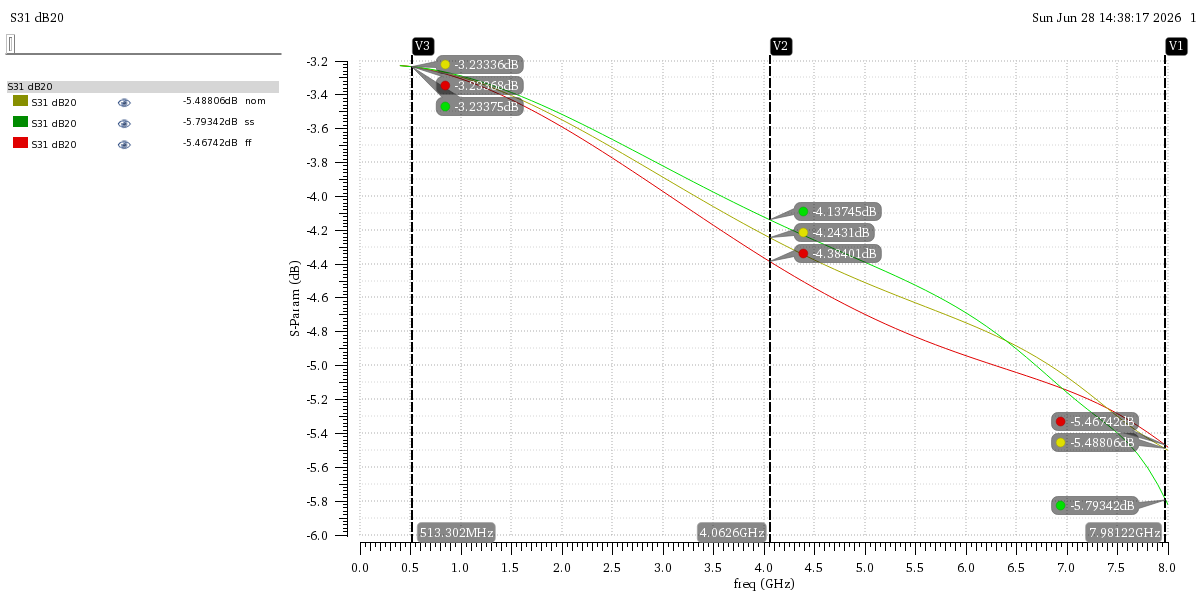
\includegraphics[width=\textwidth]{thesis_chapter_latex/figures/fig_power_divider_il_path2_corners.png}
    \caption{Power divider insertion loss, Path 2, across corners}
    \label{fig:pd_il_path2_corners}
\end{figure}

\textbf{Gain and Insertion Loss Performance} --- As demonstrated in Figures~\ref{fig:pd_il_path1_corners} and~\ref{fig:pd_il_path2_corners}, the worst-case insertion loss is 6.8~dB, which remains within the required 7~dB specification. Additionally, a gain roll-off of approximately 3~dB is observed across the band; this variation will be compensated for during the integration of the full system line-up design.

\subsection{Output Phase}
output phase is as illustrated in Figure 1.8
\begin{figure}[htbp]
    \centering
    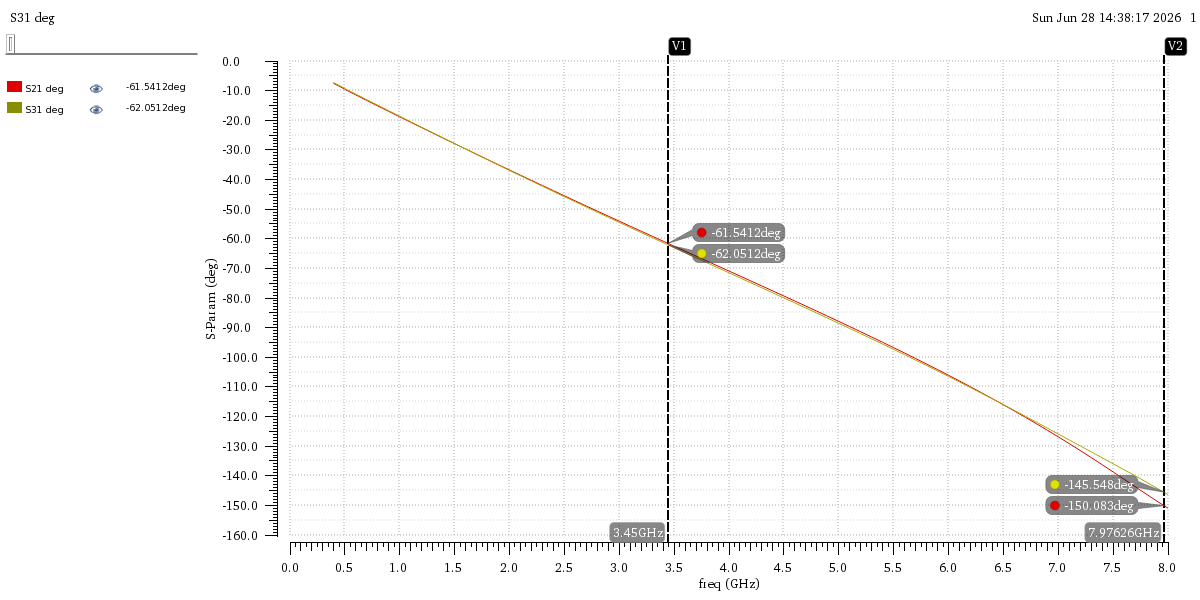
\includegraphics[width=\textwidth]{thesis_chapter_latex/figures/fig_power_divider_output_phase.png}
    \caption{Power divider output phases at nominal case}
    \label{fig:pd_output_phase}
\end{figure}

\subsection{Noise Figure}

\begin{figure}[htbp]
    \centering
    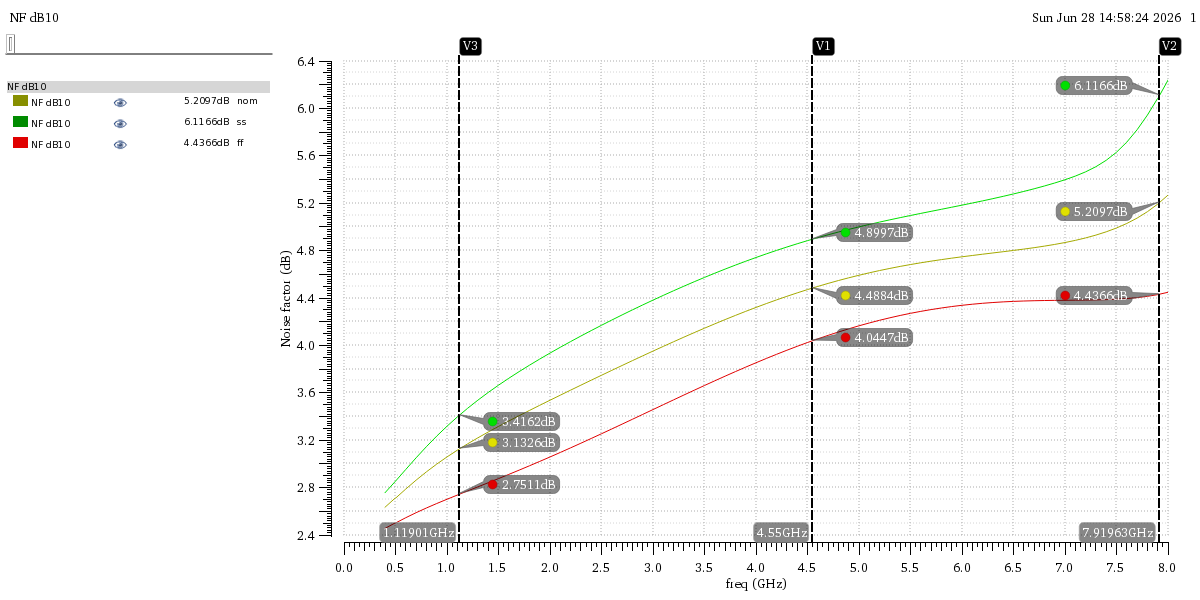
\includegraphics[width=\textwidth]{thesis_chapter_latex/figures/fig_power_divider_noise_figure.png}
    \caption{Power divider noise figure}
    \label{fig:pd_noise_figure}
\end{figure}

\textbf{Noise Figure Analysis} --- As illustrated in Figure~\ref{fig:pd_noise_figure}, the noise figure of the power divider closely tracks its insertion loss profile. This behavior is fully consistent with theoretical expectations, as the power divider is a passive network where the noise figure is fundamentally determined by its attenuation losses.

\subsection{Input Matching}

\begin{figure}[htbp]
    \centering
    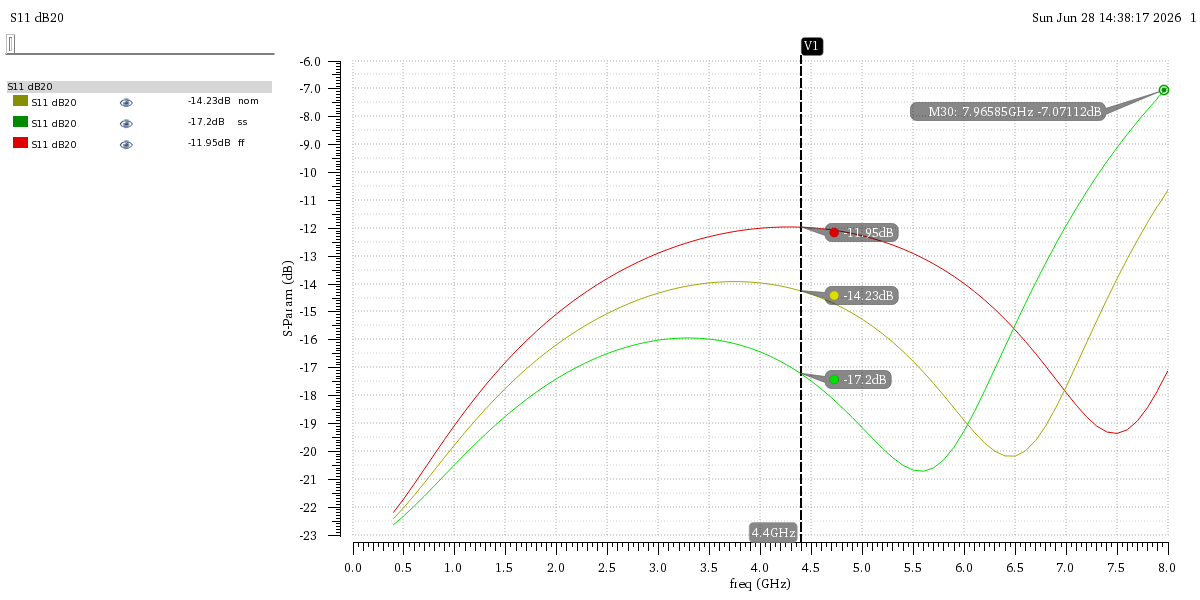
\includegraphics[width=\textwidth]{thesis_chapter_latex/figures/fig_power_divider_input_match.png}
    \caption{Power divider input match}
    \label{fig:pd_input_match}
\end{figure}

\textbf{Input Impedance Matching} --- As shown in Figure~\ref{fig:pd_input_match}, the input return loss remains below $-10$~dB across the majority of the frequency range. While the matching degrades at higher frequencies, it remains safely below the $-7$~dB threshold. This performance is acceptable since the power divider operates as an intermediate block within the system chain rather than at the primary input stage.

\subsection{Output Matching}

\begin{figure}[htbp]
    \centering
    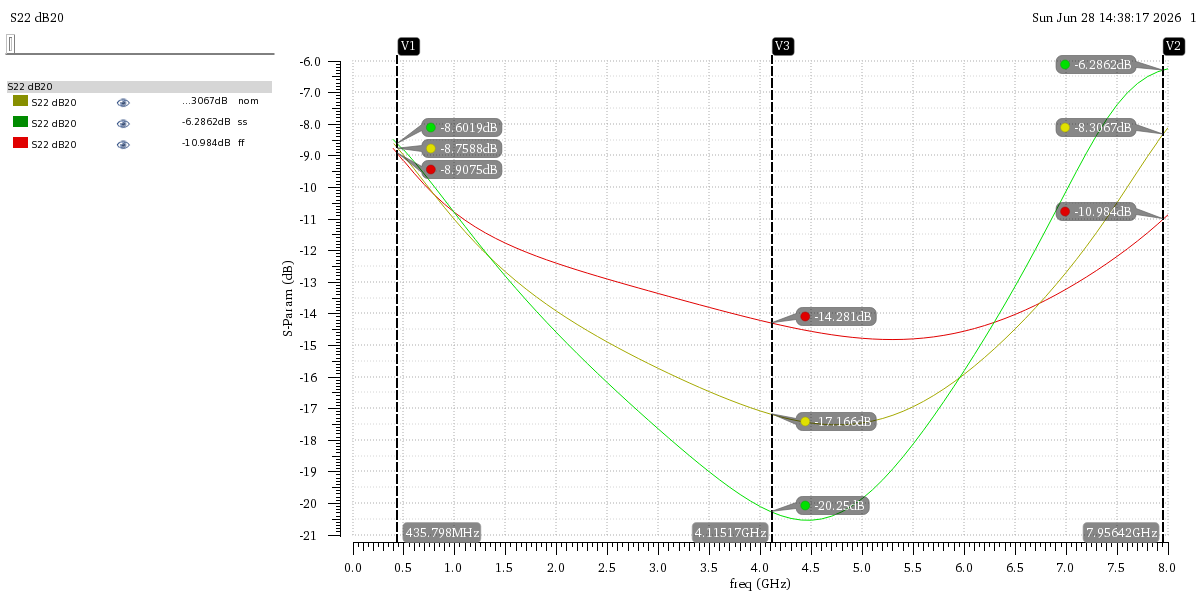
\includegraphics[width=\textwidth]{thesis_chapter_latex/figures/fig_power_divider_output_match_path1.png}
    \caption{Power divider Path 1 output match}
    \label{fig:pd_output_match_path1}
\end{figure}

\begin{figure}[htbp]
    \centering
    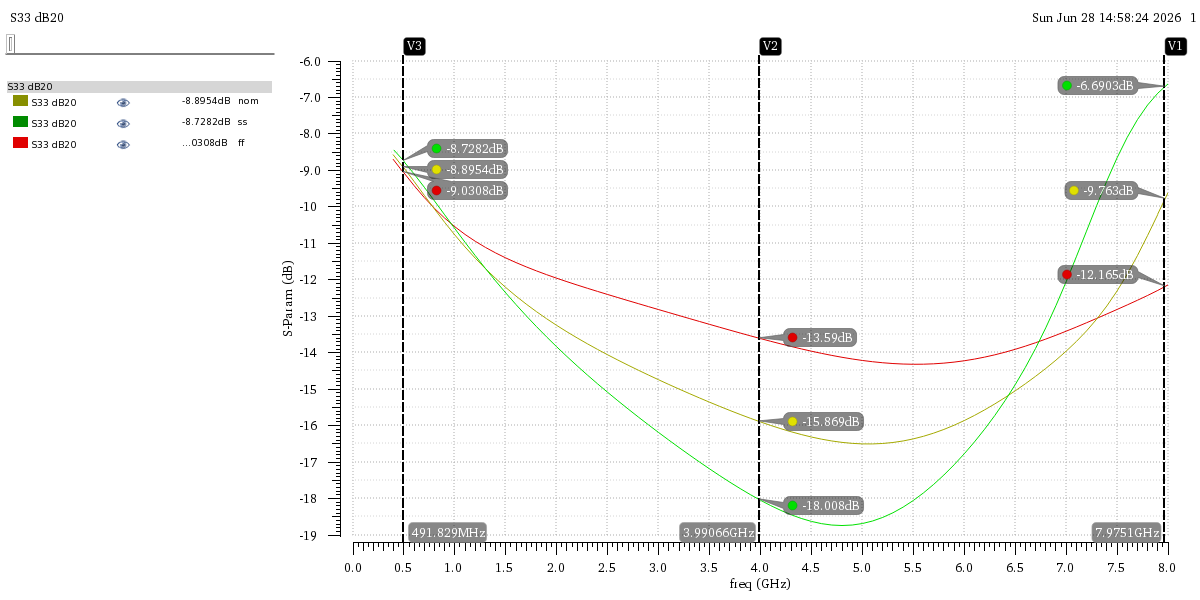
\includegraphics[width=\textwidth]{thesis_chapter_latex/figures/fig_power_divider_output_match_path2.png}
    \caption{Power divider Path 2 output match}
    \label{fig:pd_output_match_path2}
\end{figure}

\textbf{Output Impedance Matching} --- As illustrated in Figures~\ref{fig:pd_output_match_path1} and~\ref{fig:pd_output_match_path2}, the output return loss remains below $-10$~dB across the majority of the operational bandwidth, with minor degradation observed at the band edges (400~MHz and 8~GHz). Across most process corners, the matching meets the specification by remaining below $-8$~dB. The only exception is the slow-hot (SS) corner, which exhibits a marginal deviation at the upper frequency edge (7.6 to 8.0~GHz), rising to approximately $-6.3$~dB.

\subsection{Output Isolation}

\begin{figure}[htbp]
    \centering
    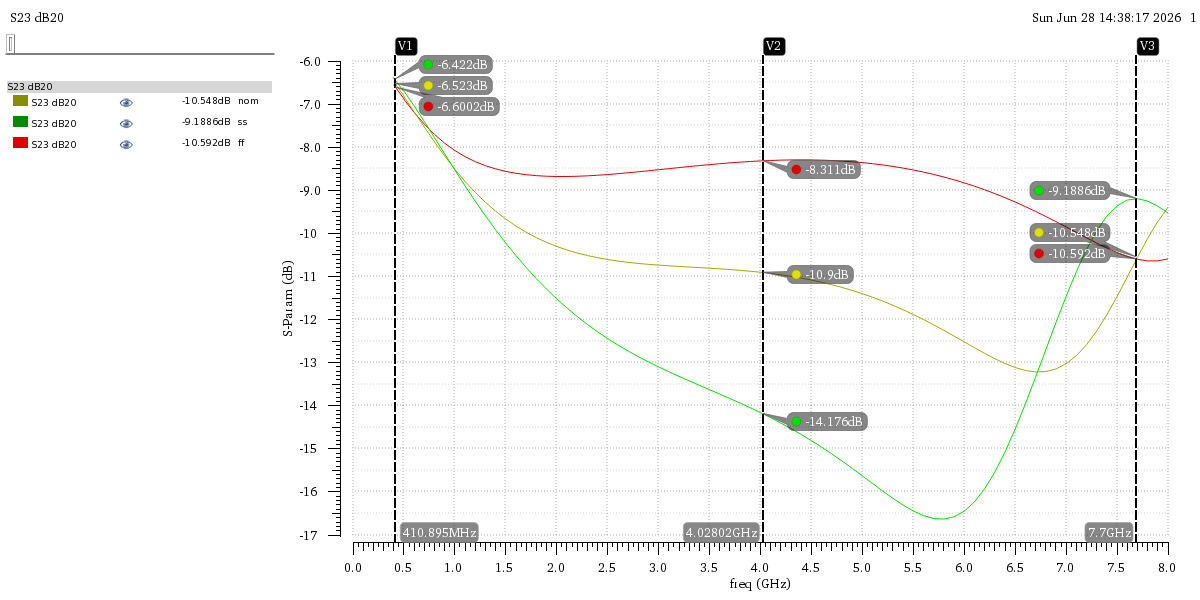
\includegraphics[width=\textwidth]{thesis_chapter_latex/figures/fig_power_divider_output_isolation.png}
    \caption{Power divider output isolation}
    \label{fig:pd_output_isolation}
\end{figure}

\textbf{Output Isolation Performance} --- As illustrated in Figure~\ref{fig:pd_output_isolation}, the port-to-port isolation successfully meets the design specification by remaining greater than 7~dB across the band, with only a marginal deviation to 6.4~dB at the lowest frequency edge. This specific isolation performance drove the selection of this topology, as it offered the optimal trade-off for ultra-wideband isolation despite requiring substantial inductive footprints. While increasing the inductor values would improve low-frequency isolation at 400~MHz, it would simultaneously degrade high-frequency performance at 8~GHz. Consequently, the component values were optimized to achieve an acceptable compromise across the entire operating range.

\subsection{Magnitude Imbalance}

\begin{figure}[htbp]
    \centering
    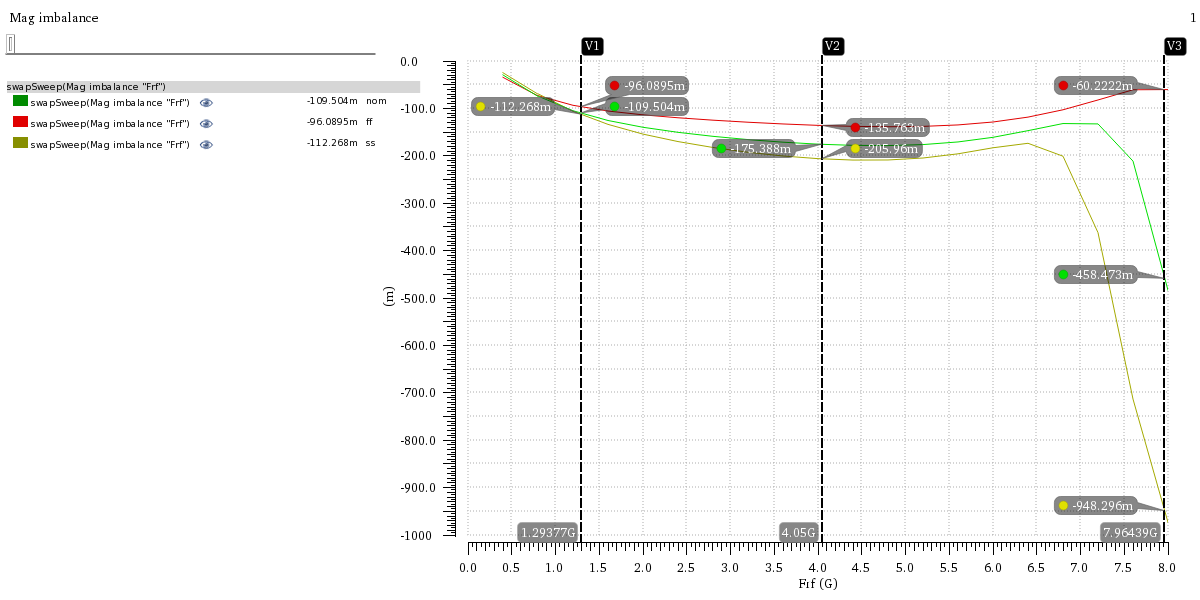
\includegraphics[width=\textwidth]{thesis_chapter_latex/figures/fig_power_divider_magnitude_imbalance.png}
    \caption{Power divider magnitude imbalance}
    \label{fig:pd_magnitude_imbalance}
\end{figure}

\textbf{Magnitude Imbalance Analysis} --- As shown in Figure~\ref{fig:pd_magnitude_imbalance}, the magnitude imbalance between the output paths remains well below 0.5~dB across nearly the entire frequency range. The only notable exception occurs at the 8~GHz band edge under the slow-hot process corner, where the imbalance marginally degrades to 1.0~dB.

\subsection{Phase Imbalance}

\begin{figure}[htbp]
    \centering
    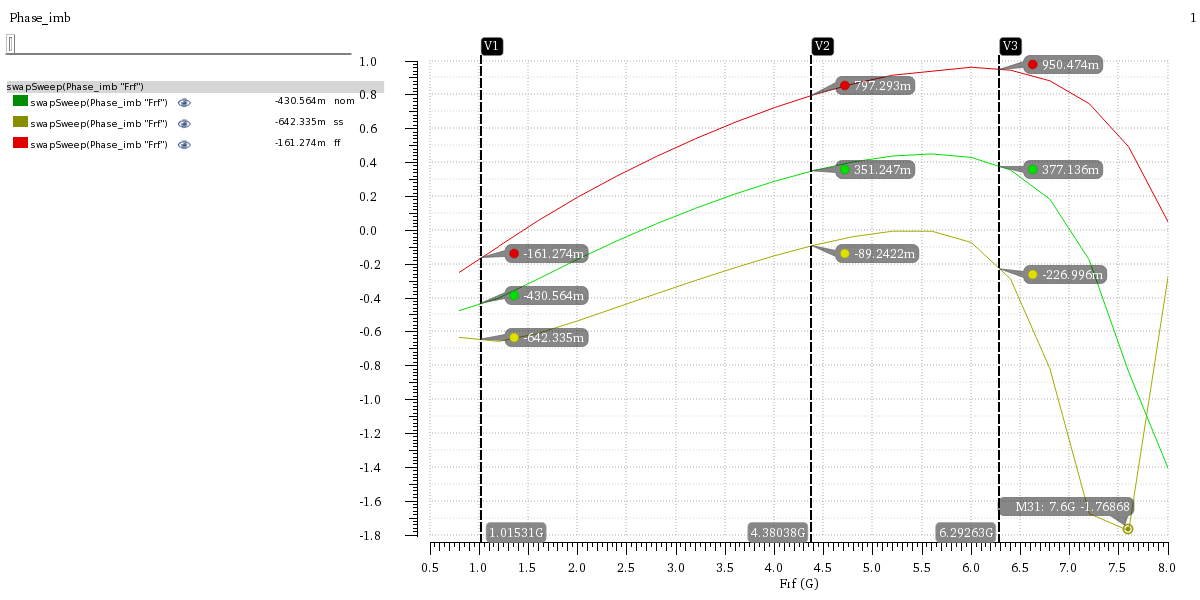
\includegraphics[width=\textwidth]{thesis_chapter_latex/figures/fig_power_divider_phase_imbalance.png}
    \caption{Power divider phase imbalance}
    \label{fig:pd_phase_imbalance}
\end{figure}

\textbf{Phase Imbalance Analysis} --- As illustrated in Figure~\ref{fig:pd_phase_imbalance}, the phase imbalance successfully satisfies the design specification, remaining below 0.5 degrees across the majority of the operating range. The worst-case deviation occurs under the slow-hot process corner at the upper band edge, where the imbalance reaches a maximum of 1.7 degrees.

\subsection{IIP3}

\begin{figure}[htbp]
    \centering
    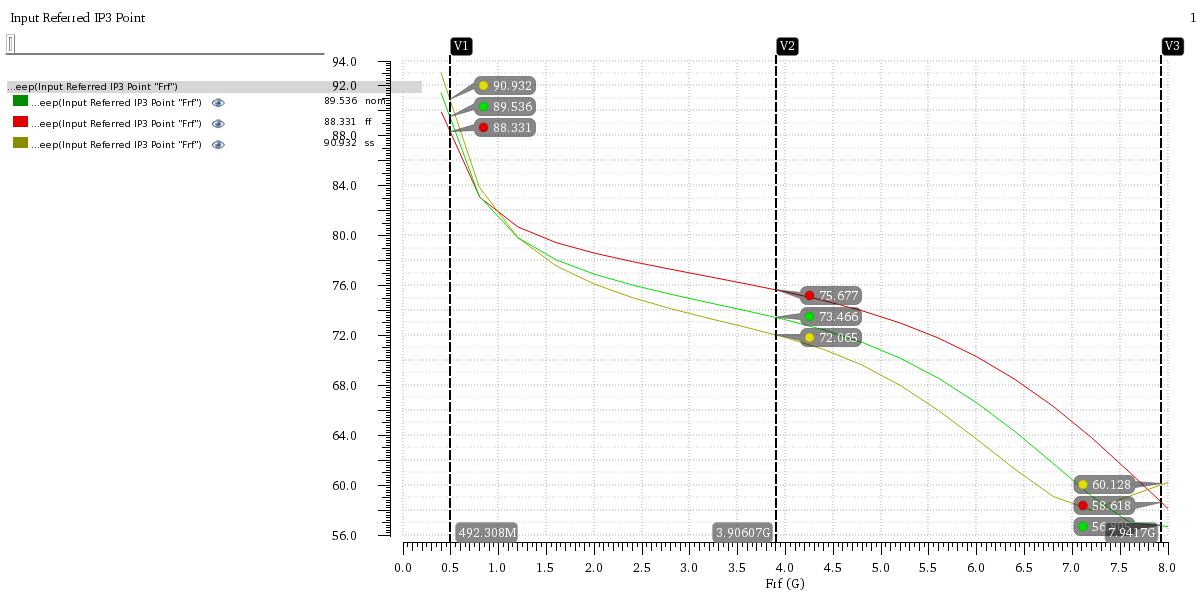
\includegraphics[width=\textwidth]{thesis_chapter_latex/figures/fig_power_divider_iip3.png}
    \caption{Power divider IIP3}
    \label{fig:pd_iip3}
\end{figure}

\textbf{Linearity Performance (IIP3)} --- As demonstrated in Figure~\ref{fig:pd_iip3}, the input third-order intercept point (IIP3) is exceptionally high across all process corners and frequencies. The worst-case IIP3 is 56~dBm, which significantly exceeds the design requirement of 40~dBm. Achieving this linearity target posed no major design challenge, as the power divider architecture consists entirely of passive components.

\section{Required versus Achieved Summary}

\begin{table}[htbp]
    \centering
    \caption{Power divider: required versus achieved performance}
    \label{tab:pd_required_vs_achieved}
    \begin{tabular}{lll}
        \toprule
        Parameter & Required Spec & Achieved \\
        \midrule
        Insertion loss      & $<$ 7~dB        & 6.8~dB \\
        Input return loss   & $<$ $-7$~dB     & $-7$~dB \\
        Input return loss   & $<$ $-7$~dB     & $-6.3$~dB \\
        Isolation           & $>$ 7~dB        & 6.4~dB \\
        Magnitude imbalance & $<$ 0.5~dB      & 0.9~dB \\
        Phase imbalance     & $<$ 0.5 degree  & 1.7 degree \\
        IIP3                & $>$ 40~dBm      & 58~dBm \\
        \bottomrule
    \end{tabular}
\end{table}

\section{References}

\begin{enumerate}
    \item[{[1]}] X.~H. Liu and Y.~S. Lin, ``Super Compact and Ultrabroadband Power Divider Using Silicon-Based Integrated Passive Device Technology,'' \emph{IEEE Transactions on Components, Packaging and Manufacturing Technology}, vol.~6, no.~12, pp.~1827--1833, Dec.~2016.
\end{enumerate}

\chapter{Mixer}

\section{Introduction}

\textbf{Frequency Translation and Mixer Fundamentals} --- Mixers are critical components in transmitter (Tx) and receiver (Rx) RF front-ends, responsible for frequency translation via the mathematical multiplication of two distinct time-domain waveforms. A mixer fundamentally utilizes three distinct signal ports (which can be configured as either single-ended or differential networks): the Radio Frequency (RF) port, the Intermediate Frequency (IF) port, and the Local Oscillator (LO) port.

\begin{itemize}
    \item \textbf{Operational Modes:} In a transmitter architecture, the mixer functions as an up-converter, translating a lower-frequency IF signal to a higher RF band. Conversely, within a receiver architecture, it serves as a down-converter, translating the high-frequency incoming RF signal back down to the IF or baseband.
    \item \textbf{Time-Varying Behavior:} Because frequency translation cannot be realized using Linear Time-Invariant (LTI) networks, mixers are fundamentally implemented as linear time-varying (LTV) blocks.
    \item \textbf{Switching Mechanics and Linearity:} Ideally, the mixer acts as a perfectly linear system with respect to the input signal path. The LO port serves strictly as a control mechanism that drives internal transistor switches, alternating between an ideal closed state (where $V_{RF} = V_{IF}$) and an open state. In practice, however, the inherent non-idealities and parasitic resistances of physical MOS transistors introduce system non-linearities.
\end{itemize}

\textbf{Harmonic Spectrum and Filtering} --- From a frequency-domain perspective, this switching mechanism is equivalent to multiplying the input signal by a periodic square wave. Because a square wave spectrum consists of a fundamental frequency alongside its odd harmonics, the desired signal conversion (the fundamental component during up-conversion, or the IF/DC component during down-conversion) must be isolated, while the unwanted harmonic products are suppressed via subsequent filtering. Consequently, while the LO port operates in a highly non-linear, large-signal switching regime, the primary signal path (RF or IF) must maintain high linearity to satisfy strict gain compression $P_{1dB}$ and third-order intermodulation $IIP3$ design constraints.

\section{Performance Parameters of Mixers}

\subsection{Noise and Linearity}

\textbf{Noise and Linearity Performance Metrics} --- Noise Figure (NF) and linearity are two critical, competing performance metrics that define the dynamic range of an RF receiver front-end.

\begin{itemize}
    \item \textbf{Noise Figure:} NF quantifies the degradation of the signal-to-noise ratio (SNR) as the signal passes through a lossy or active block, mathematically defined as:
\begin{equation}
NF = \frac{SNR_{in}}{SNR_{out}}
\end{equation}
    \item \textbf{Linearity:} This metric defines the maximum signal power the system can handle before distortion occurs, setting the upper limit of the receiver's dynamic range. While an ideal system obeys superposition and scales perfectly linearly, physical transistor non-idealities cause gain compression and intermodulation distortion.
\end{itemize}

\textbf{Receiver Chain Integration and Design Trade-offs} --- In a standard receiver chain, the down-conversion mixer follows the Low-Noise Amplifier (LNA). According to Friis' formula, the noise and non-linearities introduced by the mixer are suppressed when referred to the primary receiver input:
\begin{equation}
NF_{total} = NF_1 + \frac{NF_2 - 1}{A_{v1}^2} + \ldots
\end{equation}

Because the mixer's input-referred noise and intercept points ($IIP3$) are divided by the preceding LNA gain, down-conversion mixer design requires a careful, direct compromise between minimizing its intrinsic NF and maximizing its linearity.

Furthermore, in direct-conversion (zero-IF) receiver architectures, maximizing the second-order intercept point ($IIP2$) is critical. Second-order intermodulation products ($IM2$) generate low-frequency distortion that falls directly within the baseband spectrum, potentially corrupting the desired signal.

\subsubsection{Noise Figure}

\textbf{Mixer Noise Figure and Image Folding} --- The Noise Figure (NF) of a down-conversion mixer is fundamentally impacted by frequency translation and image folding, leading to two distinct definitions: Single-Sideband (SSB) and Double-Sideband (DSB) noise figures.

Consider an ideal, noiseless down-conversion mixer with unity gain operating in a heterodyne (IF-receiver) architecture. The frequency conversion process down-converts two distinct RF bands to the same Intermediate Frequency (IF): the desired signal band and the mirror image band located on the opposite side of the Local Oscillator (LO) tone, spaced by exactly twice $f_{IF}$.

\begin{itemize}
    \item \textbf{Signal and Noise Translation:} During down-conversion, the signal power is translated from the desired RF band to the IF band. However, uncorrelated thermal noise present at both the desired RF band and the image RF band is down-converted and folded into the exact same IF band.
    \item \textbf{SNR Degradation:} Assuming the noise spectral density is identical across both input bands, the total noise power at the IF output doubles. Because the output noise power is twice as large while the signal power is only translated from a single band, the output Signal-to-Noise Ratio ($SNR_{out}$) is exactly halved relative to the input SNR.
    \item \textbf{SSB Noise Figure:} This mandatory 3~dB reduction in SNR dictates that an internally noiseless, ideal mixer has a Single-Sideband noise figure of exactly 3~dB.
\end{itemize}

\subsubsection{Linearity}

\textbf{Mixer Linearity and Signal Strength Limits} --- Similar to amplifiers, mixers exhibit distinct limitations regarding maximum input signal power, primarily bounded by gain compression and intermodulation distortion.

\begin{itemize}
    \item \textbf{Gain Compression:} The 1-dB compression point ($P_{1dB}$) defines the input or output power level at which the actual conversion gain drops by 1~dB relative to the ideal linear gain.
    \item \textbf{Intermodulation and Intercept Points:} Non-linearities in the RF signal path cause in-band intermodulation products when two closely spaced interferers ($f_1$ and $f_2$) are present. This behavior is quantified by the input and output third-order intercept points ($IIP3$ and $OIP3$). For typical active or passive mixers, the IIP3 is generally 10~dBm or less. The resulting third-order intermodulation ($IM3$) spur frequencies at the mixer output are mathematically defined as:
\begin{equation}
f_{IM3} = 2f_1 \pm f_2 \pm f_{LO} \quad \text{or} \quad 2f_2 \pm f_1 \pm f_{LO}
\end{equation}
\end{itemize}

\textbf{Port-Specific Non-Linearity Analysis} --- The architectural impact of non-linear behavior varies significantly across the three mixer ports:

\begin{itemize}
    \item \textbf{RF Port:} Non-linearity at the RF input is highly critical. It limits the receiver's blocking performance, making the rejection of out-of-band interferers difficult.
    \item \textbf{LO Port:} Non-linearity here is generally acceptable because the LO is intentionally driven hard to operate as a periodic switch. The primary design concerns are limited to suppressing second-order harmonics and minimizing LO-to-RF/LO-to-IF leakage.
    \item \textbf{IF Port:} Non-linearity at the output stage causes self-mixing of the down-converted IF signal, which can be effectively mitigated by utilizing highly linear, symmetric active or passive loads.
\end{itemize}

\textbf{Spurious Responses (Spurs)} --- Due to the multiplication of the time-varying waveforms, mixers generate an array of cross-products originating from the fundamental frequencies and their higher-order harmonics. These mixing products create spurious responses at the output, defined by:
\begin{equation}
f_{spurs} = \pm m f_{RF} \pm n f_{LO}
\end{equation}
where $m$ and $n$ are positive integers. To prevent corruption of the desired baseband or intermediate frequency signal, these unwanted harmonic combinations must be systematically suppressed using targeted filtering networks.

\subsection{Conversion Gain (Loss)}

\textbf{Conversion Gain and Loss} --- Conversion gain (or loss) is the ratio of the desired output signal power to the input signal power (IF-to-RF power for down-conversion, or RF-to-IF for up-conversion).

\begin{itemize}
    \item \textbf{Active Mixers:} Provide a net conversion gain ($A_v > 0$~dB). While this helps suppress the noise of subsequent stages, it presents a strict trade-off with linearity and stability. Standard design practice prioritizes optimizing for low noise and high linearity over maximizing gain, as excessive gain compresses voltage headroom and reduces stability margins.
    \item \textbf{Passive Mixers:} Incur a conversion loss ($A_v < 0$~dB), but inherently offer significantly superior linearity margins (IIP3) and lower flicker (1/f) noise because they lack active DC bias currents in the signal path.
\end{itemize}

\subsection{Port-to-Port Isolation}

\textbf{Port-to-Port Isolation and Leakage} --- Ideally, each mixer port should isolate its designated frequency and suppress feedthrough from the other two ports. Real-world isolation values typically range from 30 to 50~dB.

\begin{itemize}
    \item \textbf{LO-to-RF Leakage (Most Critical):} In direct-conversion receivers, leaked LO signals can reflect back and mix with the main LO tone, causing ``self-mixing'' which generates a disruptive DC offset at baseband. Furthermore, if the leaked LO propagates backward through the LNA to the antenna, it will radiate into space, violating strict regulatory emission standards.
    \item \textbf{LO-to-IF Feedthrough:} Because the LO signal is driven at a much higher power level than the desired signal, unattenuated LO feedthrough can desensitize or saturate subsequent intermediate-frequency or baseband stages.
    \item \textbf{RF-to-LO Feedthrough:} This allows strong incoming RF interferers and out-of-band spurs to corrupt the LO signal, potentially modulating the switching core.
    \item \textbf{RF-to-IF Feedthrough:} Direct feedthrough of the RF envelope to the output can degrade the second-order intermodulation ($IIP2$) performance, presenting a major challenge in zero-IF architectures.
\end{itemize}

\section{Mixer Topologies}

\textbf{Mixer Classification Framework} --- Mixers are categorized according to three primary architectural and operational domains:

\begin{itemize}
    \item \textbf{Principle of Operation:} Mixers are classified as either \textbf{non-linear} or \textbf{commutating (switching)} topologies. Non-linear mixers---such as single-diode, single-FET, and dual-gate FET mixers---rely on the square-law characteristic of the device to generate mixing products. Commutating mixers operate as periodic switches in either the voltage or current domain; examples include the active Gilbert cell, as well as passive diode-ring and FET-ring configurations. These can be further split broadly into \textbf{active} topologies (which provide conversion gain) and \textbf{passive} topologies (which exhibit conversion loss).
    \item \textbf{Port Balance:} Based on the suppression of unwanted input signals at the output, mixers are divided into three topologies:
    \begin{itemize}
        \item \emph{Unbalanced:} No inherent isolation; both the LO and RF signals appear at the output port.
        \item \emph{Single-Balanced:} Utilizes a differential pair to inherently suppress either the LO or RF signal at the output.
        \item \emph{Double-Balanced:} Employs a fully symmetrical structure to suppress \emph{both} the LO and RF feedthrough, providing high port-to-port isolation.
    \end{itemize}
    \item \textbf{Sideband Selection:} Depending on their frequency-translation response, mixers are classified as \textbf{Upper Sideband (USB)}, \textbf{Lower Sideband (LSB)}, or \textbf{Image-Reject (USB/LSB)} mixers, which isolate or combine specific sideband spectrums relative to the LO carrier.
\end{itemize}

\section{Mixer Design Procedure}

\textbf{Mixer Architecture and Topology Selection} --- In this work, a fully differential signaling approach is implemented for the RF and BB signal paths to maximize common-mode rejection and improve overall linearity. Additionally, the LO network is driven differentially to optimize port-to-port feedthrough cancellation. By employing differential structures across all three ports, the implementation constitutes a fully double-balanced mixer configuration.

To satisfy the system line-up requirements of the receiver chain, a passive ring mixer topology was chosen based on the following architectural considerations:

\begin{itemize}
    \item \textbf{Gain Distribution:} Because the required system voltage gain is already provided by other active blocks within the receiver chain, the conversion loss of a passive topology is acceptable.
    \item \textbf{Linearity Optimization:} The high intrinsic linearity (IIP3) of the passive ring architecture is critical to achieving the stringent overall linearity specification of the entire receiver chain.
    \item \textbf{Noise Figure Impact:} Because the mixer is positioned further down the receiver chain rather than directly following the LNA, its noise contribution is heavily suppressed by the gain of the preceding stages, minimizing its impact on the total receiver noise figure.
\end{itemize}

\begin{figure}[htbp]
    \centering
    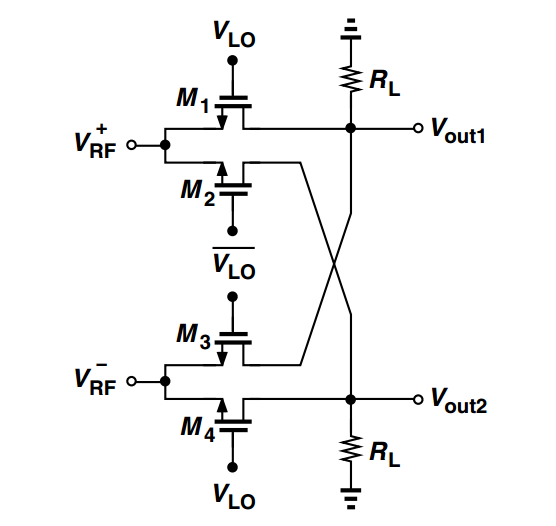
\includegraphics[width=0.7\textwidth]{thesis_chapter_latex/figures/fig_double_balanced_mixer.png}
    \caption{Double-balanced passive mixer}
    \label{fig:double_balanced_mixer}
\end{figure}

\begin{table}[htbp]
    \centering
    \caption{Mixer design specifications}
    \label{tab:mixer_design_specs}
    \begin{tabular}{ll}
        \toprule
        Specs & Required \\
        \midrule
        RF range            & 400~MHz -- 8~GHz \\
        BB range            & DC \\
        LO range            & 400~MHz -- 8~GHz \\
        Loss                & $<$ 7~dB \\
        NF                  & $<$ 7~dB \\
        IIP3                & $>$ 11~dBm \\
        IIP2                & $>$ 30~dBm \\
        LO to RF Isolation  & $>$ 40~dBc \\
        LO to BB Isolation  & $>$ 40~dBc \\
        S11                 & $<$ $-7$~dB \\
        S22                 & $<$ $-7$~dB \\
        \bottomrule
    \end{tabular}
\end{table}

\textbf{Passive Ring Mixer Design and Optimization} --- The design of the passive ring mixer begins with the strategic sizing (width and length) of the switching transistors to minimize conversion loss prior to impedance matching. Maximum available gain ($G_{max}$) simulations are initially performed to determine the optimal loss achievable under perfect matching conditions, with an ideal theoretical baseline of $-4$~dB.

\begin{itemize}
    \item \textbf{Transistor Sizing and Parasitics:} Operating as periodic switches, the transistors are characterized by their on/off resistances ($R_{on}$, $R_{off}$) and capacitances ($C_{on}$, $C_{off}$). To minimize $R_{on}$ for reduced insertion loss while lowering parasitic capacitances for enhanced isolation, the minimum channel length of 20~nm is selected. Since $R_{on} = 1/(K \cdot V_{ov})$ is inversely proportional to the channel width $W$, while parasitic capacitance scales linearly with $W$, an intermediate width is chosen as an optimal compromise. Furthermore, the layout employs a multi-finger configuration with reduced finger widths to lower gate resistance and minimize substrate losses.
    \item \textbf{Architectural Note:} In this direct-conversion architecture, the mixer translates the RF signal directly to baseband (BB) rather than an intermediate frequency (IF).
\end{itemize}

\textbf{Linearity and LO Drive Optimization} --- Circuit linearity constraints---including gain compression and intermodulation products---are satisfied by optimizing the voltage swing and biasing at the LO switching port.

\section{Mixer's Core Layout}

\begin{figure}[htbp]
    \centering
    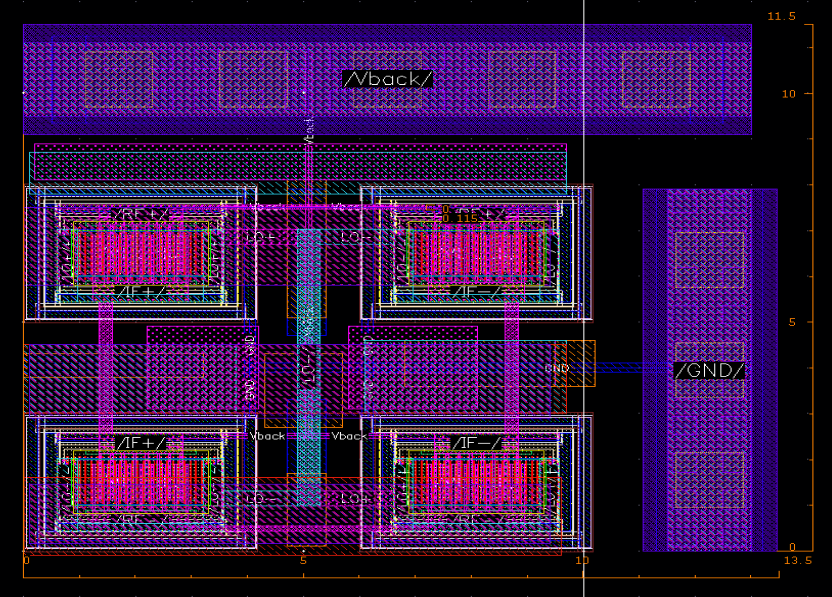
\includegraphics[width=0.6\textwidth]{thesis_chapter_latex/figures/fig_mixer_layout.png}
    \caption{Mixer layout}
    \label{fig:mixer_layout}
\end{figure}

\textbf{Mixer Layout Design} --- As illustrated in Figure~\ref{fig:mixer_layout}, the mixer layout is executed with strict geometric symmetry to ensure precise isolation across the LO, RF, and baseband (BB) ports. This symmetrical arrangement minimizes phase and amplitude imbalances while maximizing port-to-port isolation. Additionally, a dense grid of dummy metal fills is strategically incorporated throughout the layout to satisfy global density and manufacturing rules for Design Rule Checking (DRC) without corrupting the critical signal paths.

\section{Mixer's Results}

\subsection{Input Matching}

\begin{figure}[htbp]
    \centering
    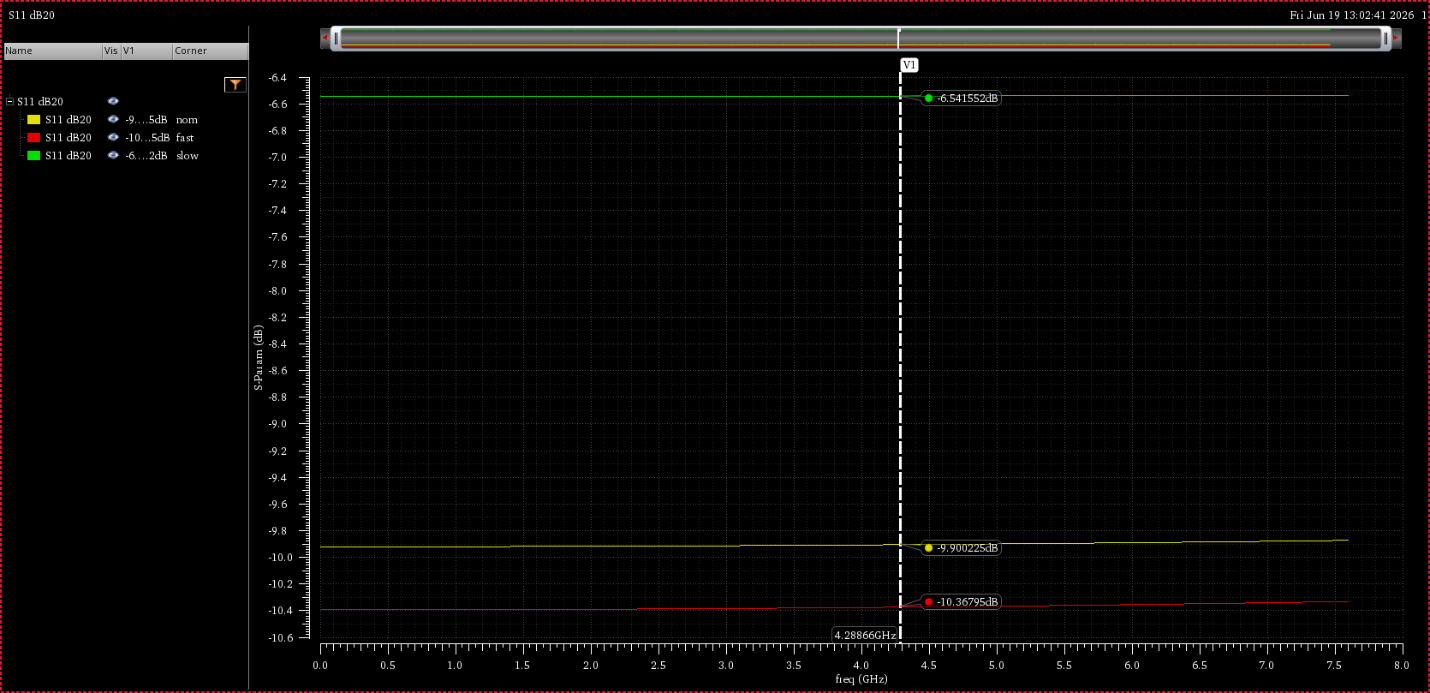
\includegraphics[width=\textwidth]{thesis_chapter_latex/figures/fig_mixer_rf_return_loss.png}
    \caption{Mixer RF port return loss across corners}
    \label{fig:mixer_rf_return_loss}
\end{figure}

\textbf{RF Port Return Loss} --- The RF port matching satisfies the return loss specification across nearly all process and temperature corners. The sole exception occurs at the slow-hot (SH) corner, where the return loss reaches 6.5~dB---falling slightly short of the strict 7~dB design target.

\subsection{Output Matching}

\begin{figure}[htbp]
    \centering
    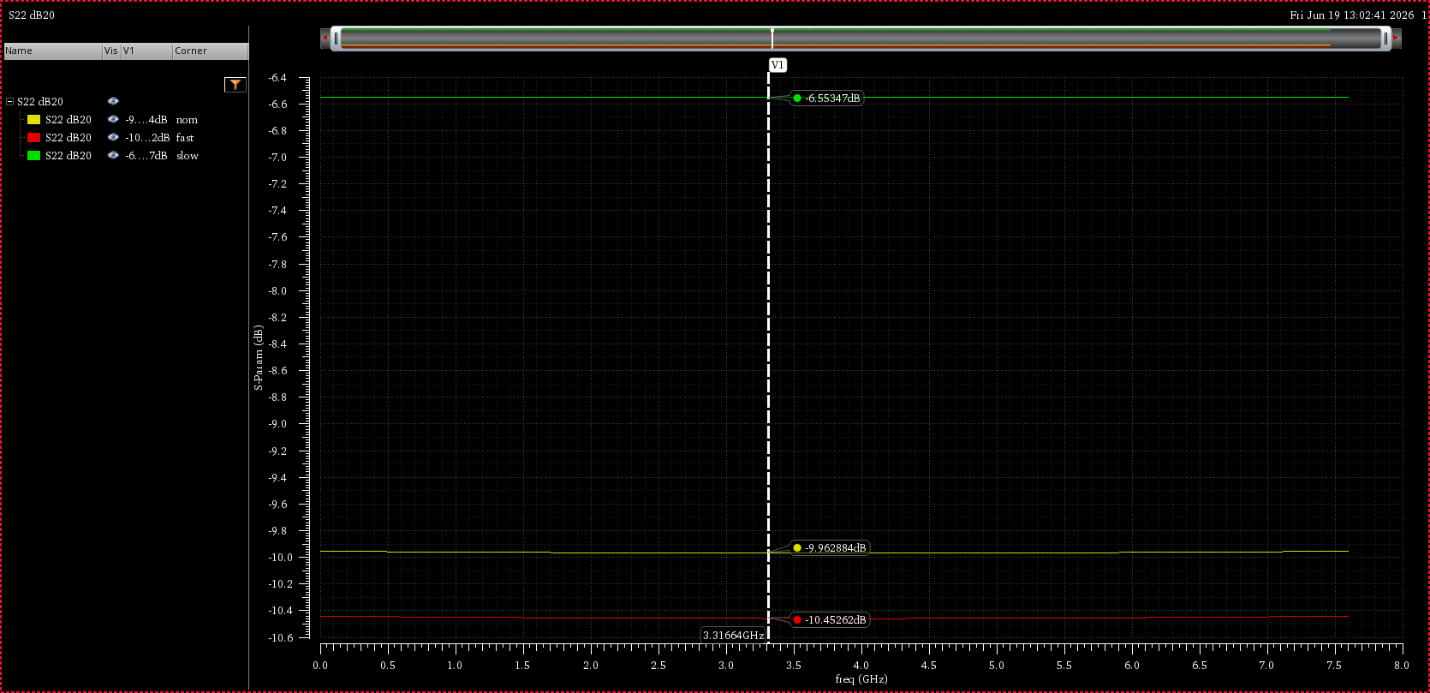
\includegraphics[width=\textwidth]{thesis_chapter_latex/figures/fig_mixer_bb_return_loss.png}
    \caption{Mixer BB port return loss across corners}
    \label{fig:mixer_bb_return_loss}
\end{figure}

\textbf{BB Port Return Loss} --- The BB port matching satisfies the return loss specification across nearly all process and temperature corners. The sole exception occurs at the slow-hot (SH) corner, where the return loss reaches 6.5~dB---falling slightly short of the strict 7~dB design target.

\subsection{Conversion Gain}

\begin{figure}[htbp]
    \centering
    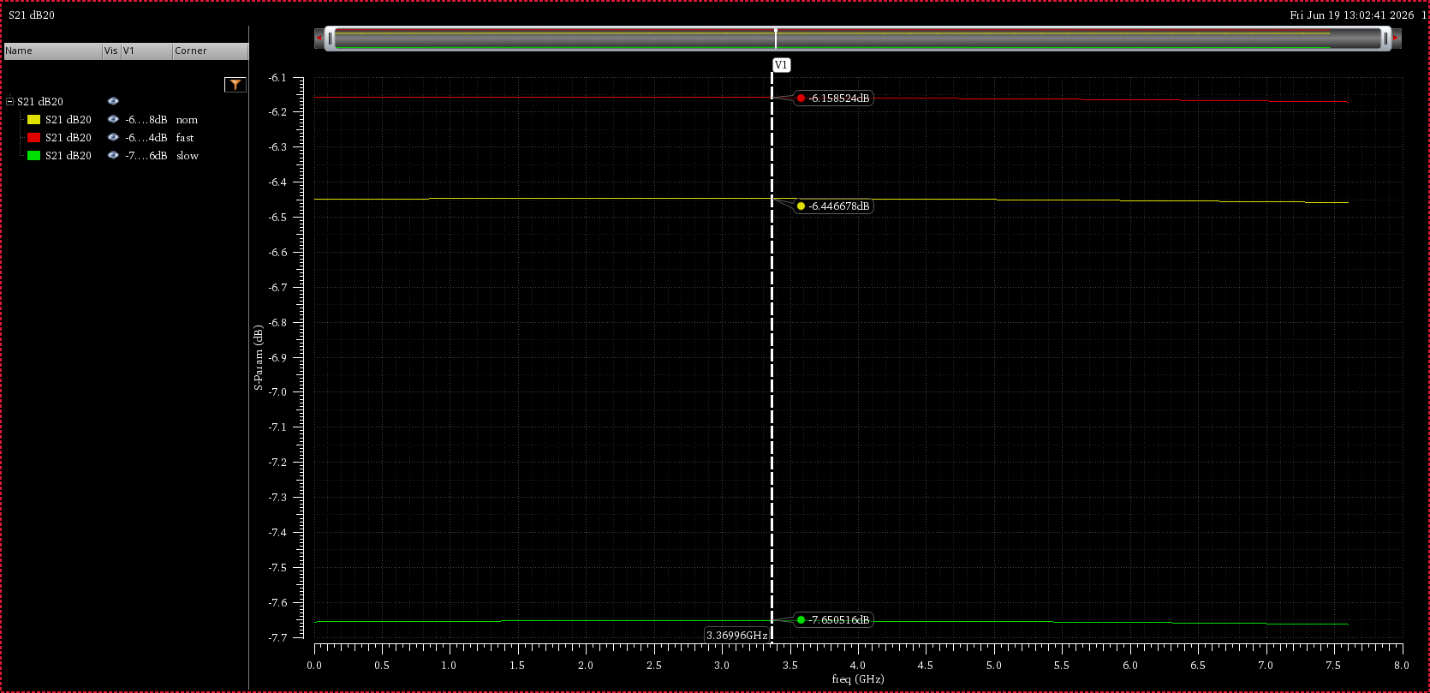
\includegraphics[width=\textwidth]{thesis_chapter_latex/figures/fig_mixer_conversion_gain.png}
    \caption{Mixer conversion gain across corners}
    \label{fig:mixer_conversion_gain}
\end{figure}

\textbf{Conversion Loss Performance} --- The mixer's conversion gain satisfies the required specification of better than $-7$~dB across the entire frequency range and nearly all process corners. The only deviation occurs at the slow-hot (SH) corner, where the gain drops slightly to $-7.6$~dB. This minor deviation is acceptable because any marginal gain deficit can be easily compensated for by adjusting the gain profile of other active blocks within the receiver chain. Furthermore, the conversion gain exhibits no high-frequency roll-off across the band, which provides an ideal, flat response for the overall system line-up calculations.

\subsection{Noise Figure}

\begin{figure}[htbp]
    \centering
    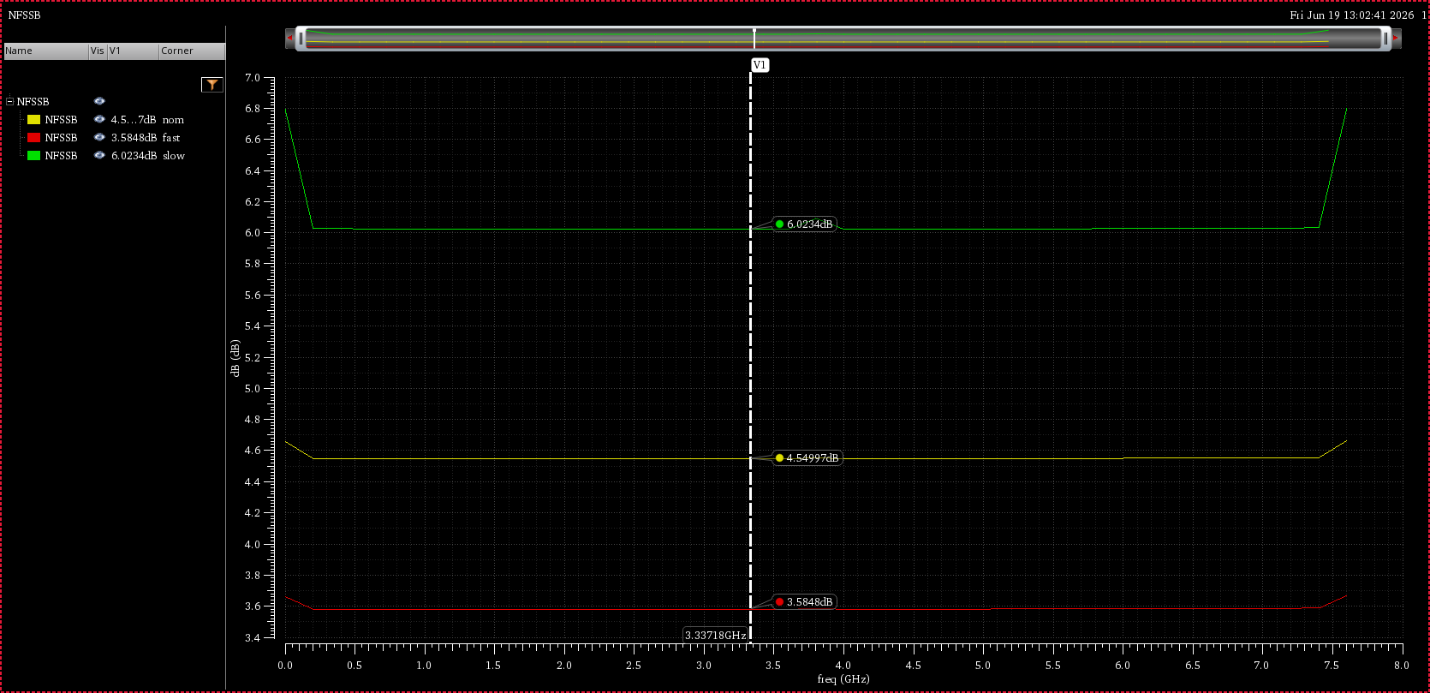
\includegraphics[width=\textwidth]{thesis_chapter_latex/figures/fig_mixer_noise_figure.png}
    \caption{Noise figure vs. RF frequency across corners}
    \label{fig:mixer_noise_figure}
\end{figure}

\textbf{Noise Figure Performance} --- The mixer's Noise Figure (NF) remains consistently below the 7~dB specification threshold across the entire operating frequency range and all simulated process and temperature corners.

\subsection{IIP3}

\begin{figure}[htbp]
    \centering
    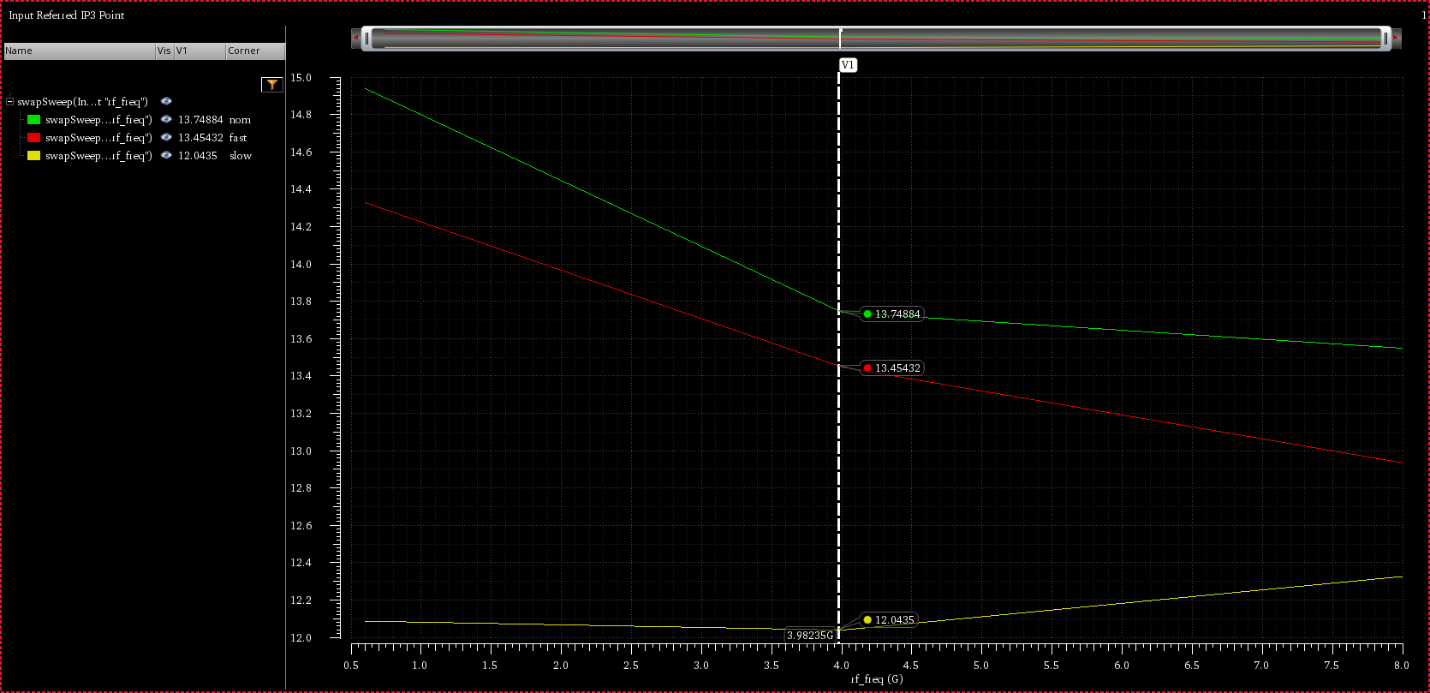
\includegraphics[width=\textwidth]{thesis_chapter_latex/figures/fig_mixer_iip3.png}
    \caption{Mixer IIP3 vs. RF frequency across corners}
    \label{fig:mixer_iip3}
\end{figure}

\textbf{Linearity and IIP3 Performance} --- The mixer satisfies the stringent linearity specification across all simulated process corners and the entire 400~MHz to 8~GHz RF operating frequency range. Against the design target of IIP3~$>$~11~dBm, the circuit maintains excellent linearity margins, achieving a minimum simulated IIP3 of 12~dBm under the worst-case corner conditions. This robust linearity profile prevents in-band intermodulation distortion from strong blockers, ensuring the necessary dynamic range for the wideband receiver front-end.

\subsection{IIP2}

\begin{figure}[htbp]
    \centering
    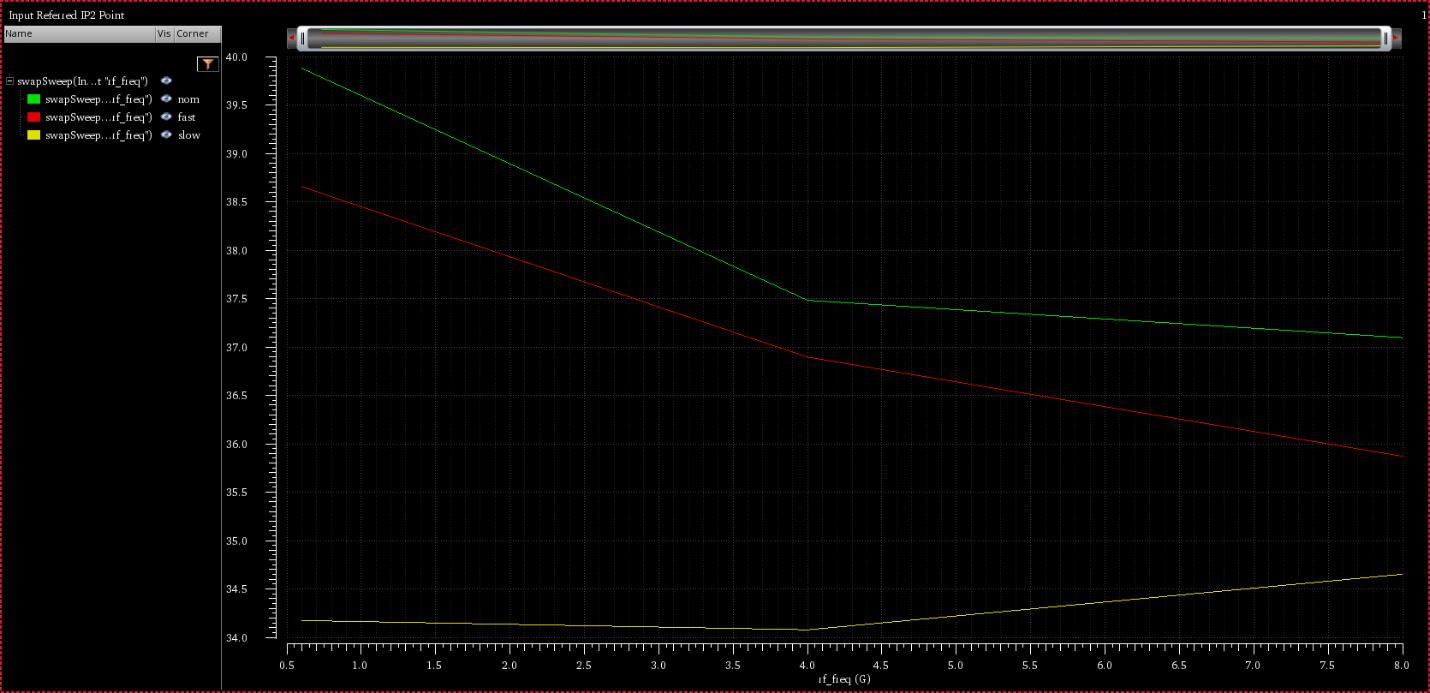
\includegraphics[width=\textwidth]{thesis_chapter_latex/figures/fig_mixer_iip2.png}
    \caption{Mixer IIP2 vs. RF frequency across corners}
    \label{fig:mixer_iip2}
\end{figure}

\textbf{IIP2 Distortion Performance} --- The additional IIP2 specification required for the direct-conversion baseband mixer is successfully achieved across all process corners and the full RF frequency range. The circuit provides a robust margin against second-order intermodulation distortion (IM2), demonstrating a worst-case minimum IIP2 of 34~dBm, which comfortably exceeds the stringent 30~dBm design target. This high level of second-order linearity prevents out-of-band blocker envelopes from down-converting as low-frequency distortion directly into the baseband spectrum.

\subsection{IP1dB}

\begin{figure}[htbp]
    \centering
    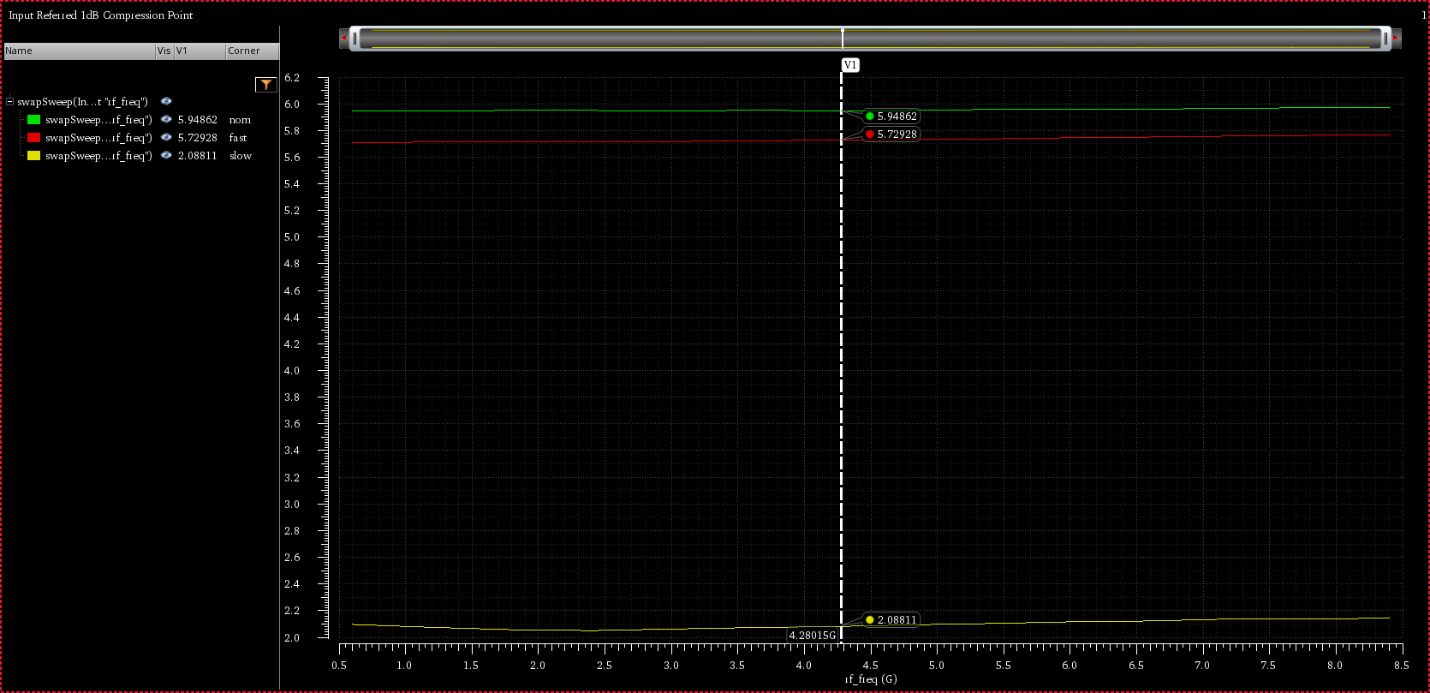
\includegraphics[width=\textwidth]{thesis_chapter_latex/figures/fig_mixer_ip1db.png}
    \caption{IP1dB vs. RF frequency across corners}
    \label{fig:mixer_ip1db}
\end{figure}

The input 1-dB compression point (IP1dB) tracks the simulated third-order intercept performance according to the classic theoretical relationship, sitting approximately 10~dB below the IIP3. This behavior satisfies the system input compression requirements across all operational conditions, demonstrating a worst-case minimum IP1dB of $+2$~dBm under the tightest corner constraints.

\subsection{LO to RF Isolation}

\begin{figure}[htbp]
    \centering
    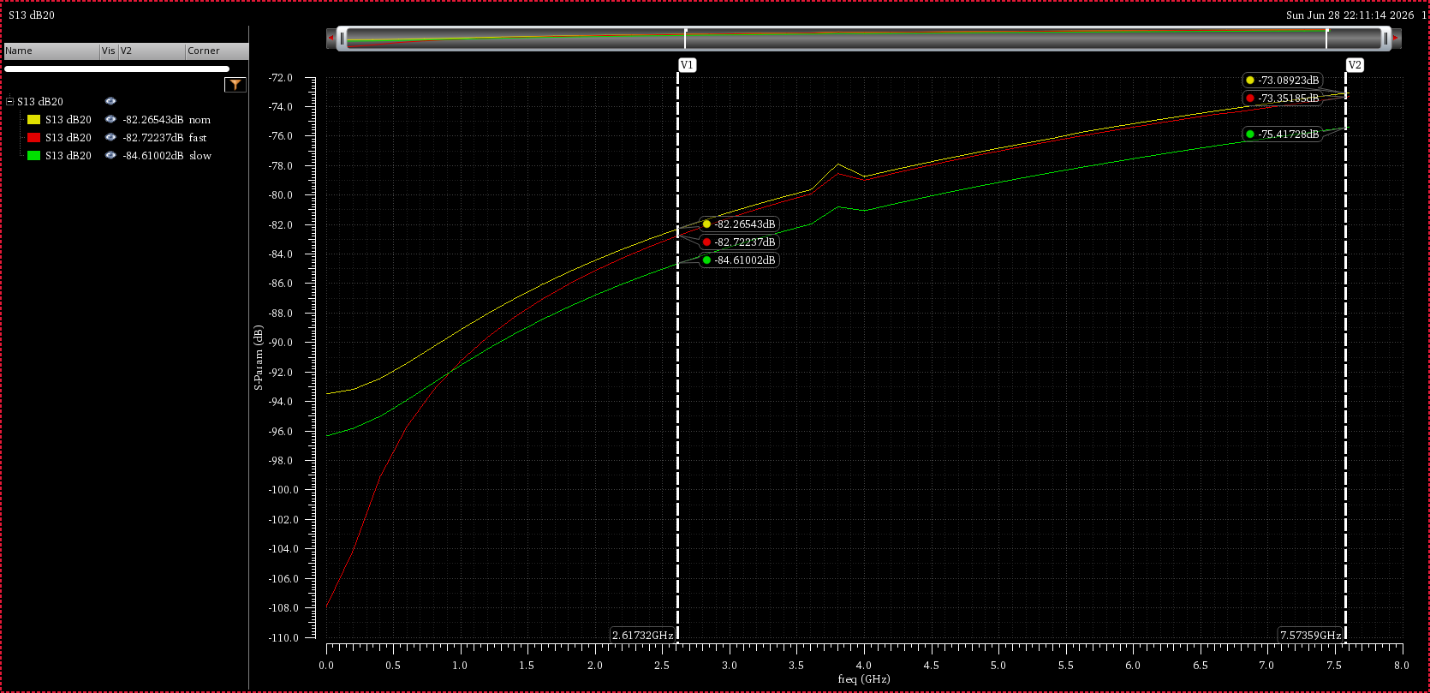
\includegraphics[width=\textwidth]{thesis_chapter_latex/figures/fig_mixer_lo_rf_isolation.png}
    \caption{LO to RF isolation across corners}
    \label{fig:mixer_lo_rf_isolation}
\end{figure}

\textbf{LO-to-RF Isolation} --- Due to the highly symmetrical geometric layout design, the mixer achieves exceptional LO-to-RF isolation across all ports. It demonstrates a worst-case minimum isolation of 73~dB across all simulated conditions, comfortably exceeding the strict system design requirement of 40~dB. This high attenuation minimizes LO leakage toward the RF port, successfully preventing self-mixing DC offsets and unauthorized antenna radiation across the wideband spectrum.

\subsection{LO to BB Isolation}

\begin{figure}[htbp]
    \centering
    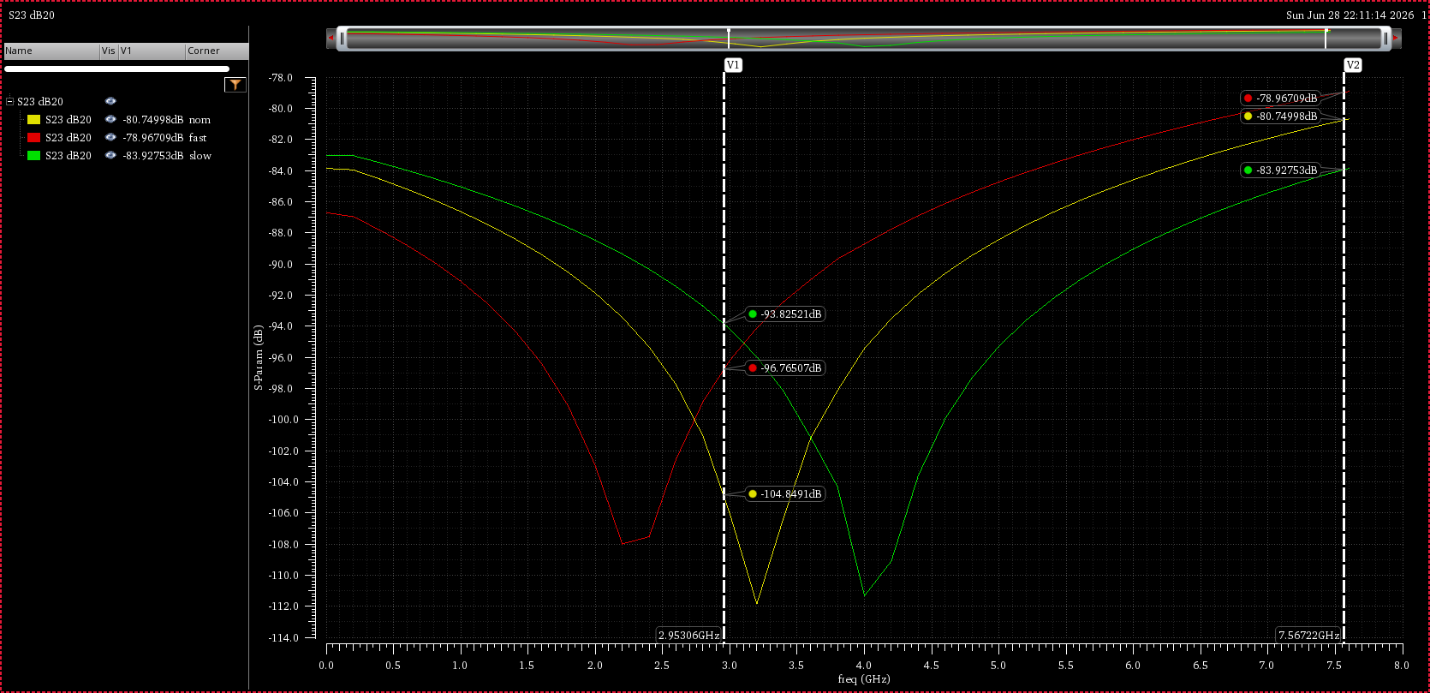
\includegraphics[width=\textwidth]{thesis_chapter_latex/figures/fig_mixer_lo_bb_isolation.png}
    \caption{LO to BB isolation across corners}
    \label{fig:mixer_lo_bb_isolation}
\end{figure}

\textbf{LO-to-BB Isolation} --- Due to the highly symmetrical geometric layout design, the mixer achieves exceptional LO-to-BB isolation across all ports. It demonstrates a worst-case minimum isolation of 78~dB across all simulated conditions, comfortably exceeding the strict system design requirement of 40~dB. This high attenuation minimizes LO leakage toward the BB port.

\section{Comparison with Previous Results}

\begin{table}[htbp]
    \centering
    \caption{Mixer: required versus achieved performance}
    \label{tab:mixer_required_vs_achieved}
    \begin{tabular}{lll}
        \toprule
        Specs               & Required          & Achieved \\
        \midrule
        RF range            & 400~MHz -- 8~GHz  & 400~MHz -- 8~GHz \\
        BB range            & DC                 & DC \\
        LO range            & 400~MHz -- 8~GHz  & 400~MHz -- 8~GHz \\
        Loss                & $<$ 7~dB           & 7.65~dB \\
        NF                  & $<$ 7~dB           & 6~dB \\
        IIP3                & $>$ 11~dBm         & 12~dBm \\
        IIP2                & $>$ 30~dBm         & 34~dBm \\
        LO to RF Isolation  & $>$ 40~dBc         & 73~dBc \\
        LO to BB Isolation  & $>$ 40~dBc         & 78~dBc \\
        S11                 & $<$ $-7$~dB        & $-6.55$~dB \\
        S22                 & $<$ $-7$~dB        & $-6.55$~dB \\
        \bottomrule
    \end{tabular}
\end{table}

\chapter{Saturation Amplifier (LO Buffer)}

\section{Introduction}

\textbf{LO Buffer and Amplification Stage} --- To deliver the large voltage swing required to drive the passive mixer's switching core, a dedicated LO buffer amplifier chain is implemented. Maintaining a highly symmetric LO waveform is critical; any rise/fall time asymmetry degrades balanced switch operation, which directly increases the mixer's noise figure and worsens the baseband second-order intermodulation (IIP2) performance due to common-mode mismatch.

The primary design objective of this buffer is to efficiently drive an effective capacitive load of 11~fF through a cascaded chain of inverters. The total number of inverter stages in this tapered chain is optimized to achieve the required voltage swing and sharp switching edges while minimizing propagation delay and power consumption.

\section{Design Procedure}

\textbf{Inverter Chain Scaling and Optimization} --- To maximize switching speeds and minimize rise and fall times ($t_{LH}$, $t_{HL}$), the final buffer stage requires large transistor aspect ratios ($W/L$). However, scaling up the output transistors proportionally increases their input gate capacitance, creating a heavy load for the preceding stage.

To manage this large capacitive load without degrading speed, a tapered chain of scaled inverters is inserted between the signal source and the mixer switches. By progressively increasing the FET sizes from the input toward the final load by a constant sizing factor, the capacitive load is distributed across multiple stages. This optimized scaling maintains sharp switching edges and minimizes the overall propagation delay of the LO buffer.

\begin{figure}[htbp]
    \centering
    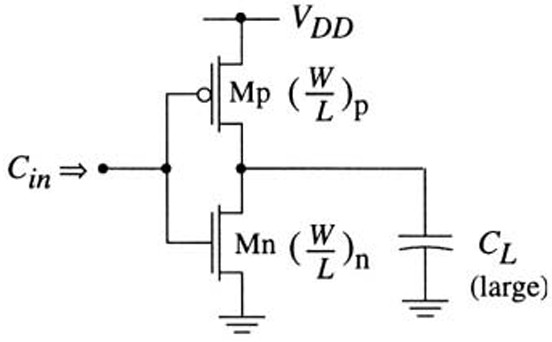
\includegraphics[width=0.7\textwidth]{thesis_chapter_latex/figures/fig_inverter_capacitive_load.jpg}
    \caption{Inverter driving a large capacitive load}
    \label{fig:inverter_capacitive_load}
\end{figure}

\begin{figure}[htbp]
    \centering
    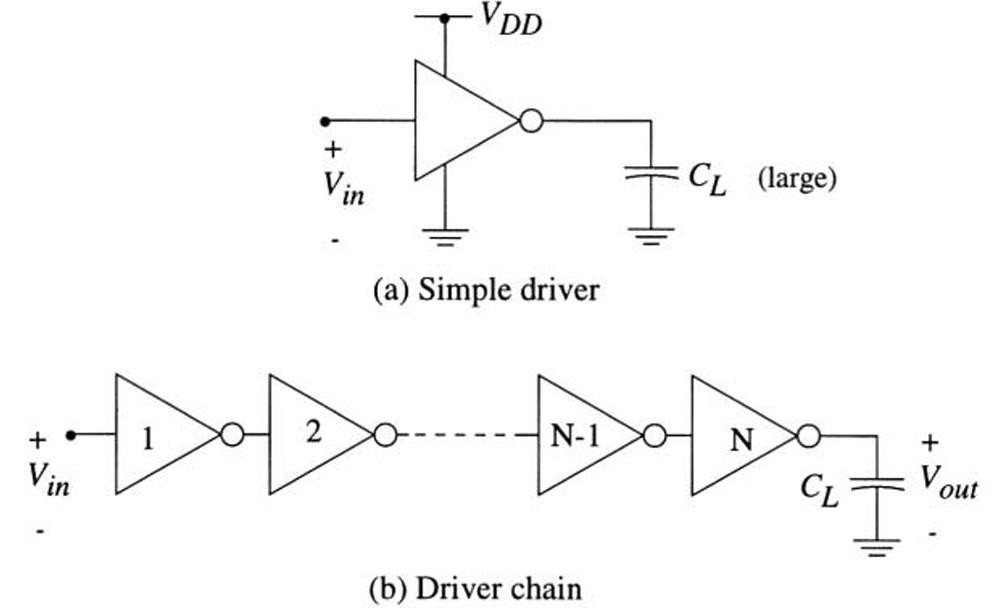
\includegraphics[width=0.85\textwidth]{thesis_chapter_latex/figures/fig_inverter_chain.jpg}
    \caption{Inverter chain}
    \label{fig:inverter_chain}
\end{figure}

\textbf{Multi-Stage Tapered Inverter Scaling} --- To systematically drive the heavy switching load, the buffer utilizes a monotonically scaled inverter chain. Inverter~1 serves as the base reference stage with a known, minimum aspect ratio denoted as $(W/L)_1$, which represents both the NMOS and PMOS base geometry sizing. The downstream stages are scaled upward sequentially such that:
\begin{equation}
(W/L)_1 < (W/L)_2 < (W/L)_3 < \ldots < (W/L)_N
\end{equation}

In this configuration, Inverter~1 features the smallest, lowest-capacitance FETs to minimize input loading, while the final stage, Inverter~$N$, features the largest geometry to source the required current. The relative geometric growth of any intermediate stage $\alpha$ (where $\alpha$ is between 2 and $N$) is governed by a scaling factor $S_\alpha$ (where $S_\alpha > 1$), defining the progressive sizing relationship:
\begin{equation}
(W/L)_\alpha = S_\alpha \cdot (W/L)_1
\end{equation}

This progressive scaling ensures that each intermediate stage provides a balanced step-up in current-driving capability, preventing any single stage from bottlenecking the signal path.

To ensure balanced switching and symmetrical waveforms, the PMOS transistor width is set to double the NMOS width ($W_p = 2 \cdot W_n$). This ratio compensates for the lower mobility of holes relative to electrons, effectively matching the pull-up and pull-down driving strengths to achieve approximately equal rise and fall times.

The optimal number of inverter stages was determined through iterative simulation and trial-and-error analysis. While a 3-to-4 stage configuration is theoretically ideal for minimizing total propagation delay when driving this capacitive load, a \textbf{3-stage chain} was selected to optimize the layout area and power trade-off. The stages are progressively scaled using a fixed tapering factor of 3, resulting in a strict geometric sizing ratio of \textbf{1:3:9} from the input stage to the final mixer driver.

\section{LO Buffer Requirements with Mixer Integration}

\begin{table}[htbp]
    \centering
    \caption{LO buffer requirements with mixer integration}
    \label{tab:lobuffer_specs}
    \begin{tabular}{ll}
        \toprule
        Spec & Required \\
        \midrule
        S11  & $<$ $-7$~dB \\
        S22  & $<$ $-7$~dB \\
        S21  & $>$ $-7$~dB \\
        IIP3 & $>$ 11~dBm \\
        \bottomrule
    \end{tabular}
\end{table}

\section{LO Buffer Layout}

\begin{figure}[htbp]
    \centering
    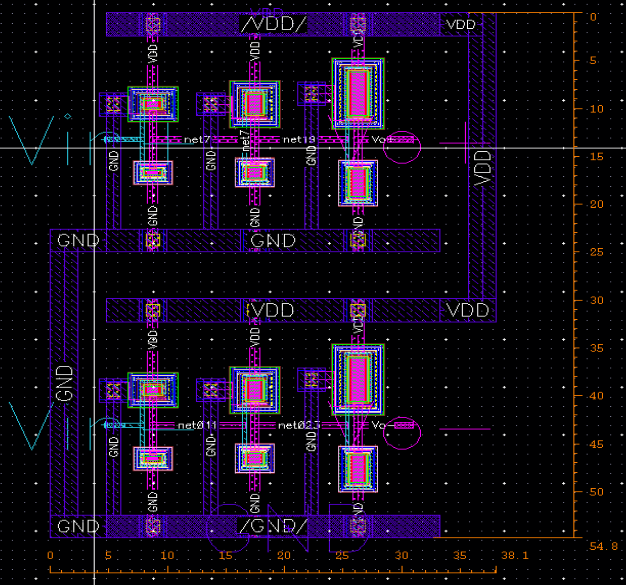
\includegraphics[width=0.6\textwidth]{thesis_chapter_latex/figures/fig_lobuffer_layout.png}
    \caption{LO buffer layout}
    \label{fig:lobuffer_layout}
\end{figure}

\begin{equation}
\text{Area} = 0.0381 \times 0.0548 = 0.002088~\text{mm}^2
\end{equation}

\section{LO Buffer Integrated with Mixer: Results}

\subsection{RF Port Return Loss}

\begin{figure}[htbp]
    \centering
    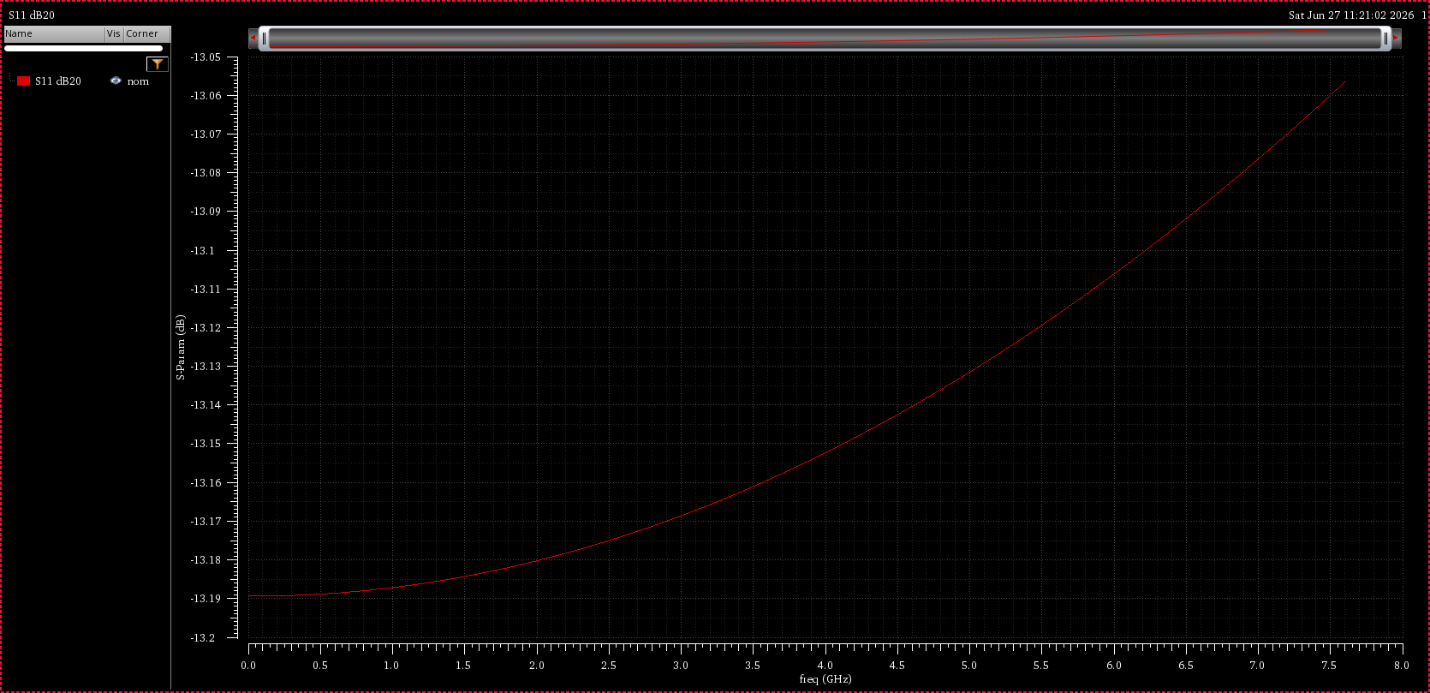
\includegraphics[width=\textwidth]{thesis_chapter_latex/figures/fig_lobuffer_rf_return_loss_nominal.png}
    \caption{RF port return loss, nominal case}
    \label{fig:lobuffer_rf_return_loss_nominal}
\end{figure}

\begin{figure}[htbp]
    \centering
    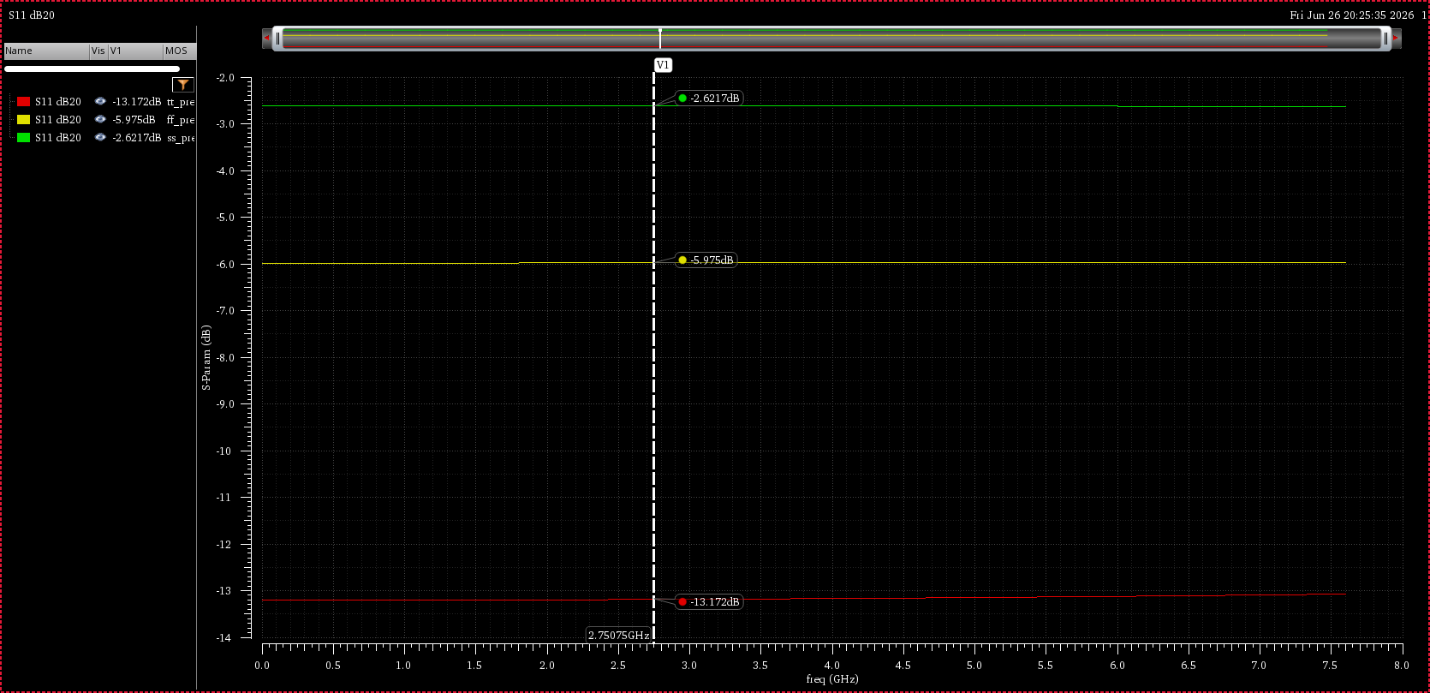
\includegraphics[width=\textwidth]{thesis_chapter_latex/figures/fig_lobuffer_rf_return_loss_corners.png}
    \caption{RF port return loss across corners}
    \label{fig:lobuffer_rf_return_loss_corners}
\end{figure}

\textbf{RF Port Return Loss} --- The RF port return loss successfully satisfies the target specifications across nearly all process and temperature corners. However, a significant failure occurs at the slow-hot (SH) corner, where the return loss drops to just 2~dB.

\subsection{BB Port Return Loss}

\begin{figure}[htbp]
    \centering
    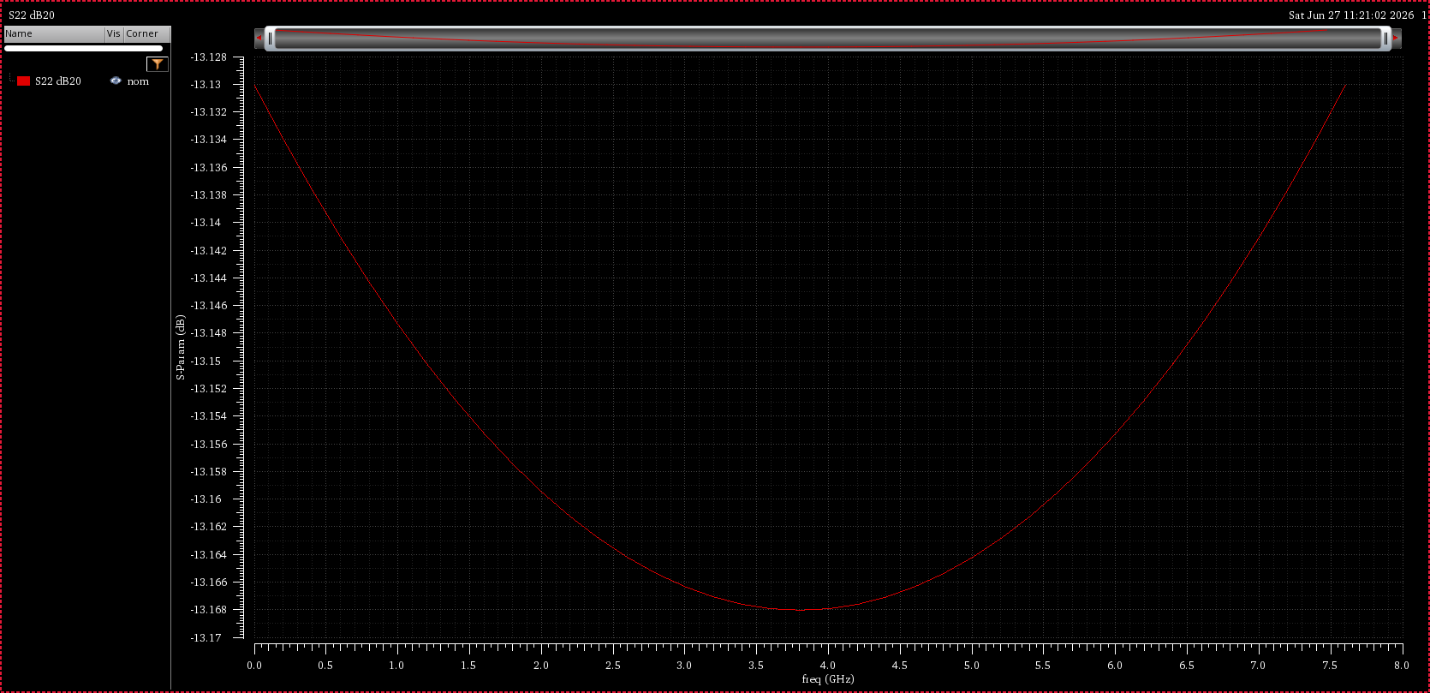
\includegraphics[width=\textwidth]{thesis_chapter_latex/figures/fig_lobuffer_bb_return_loss_nominal.png}
    \caption{BB return loss, typical case}
    \label{fig:lobuffer_bb_return_loss_nominal}
\end{figure}

\begin{figure}[htbp]
    \centering
    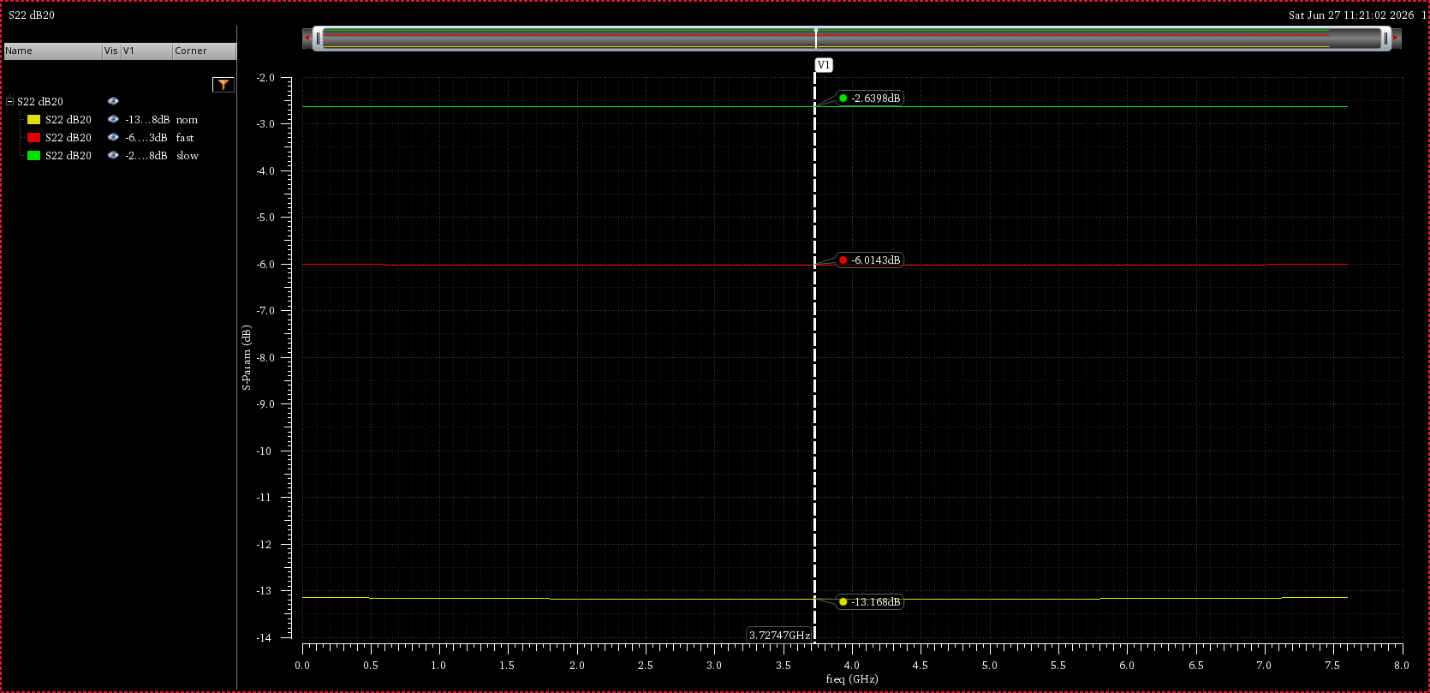
\includegraphics[width=\textwidth]{thesis_chapter_latex/figures/fig_lobuffer_bb_return_loss_corners.png}
    \caption{BB return loss across corners}
    \label{fig:lobuffer_bb_return_loss_corners}
\end{figure}

\textbf{BB Port Return Loss} --- The BB port return loss successfully satisfies the target specifications across nearly all process and temperature corners. However, a significant failure occurs at the slow-hot (SH) corner, where the return loss drops to just 2~dB.

\subsection{Mixer Conversion Gain}

\begin{figure}[htbp]
    \centering
    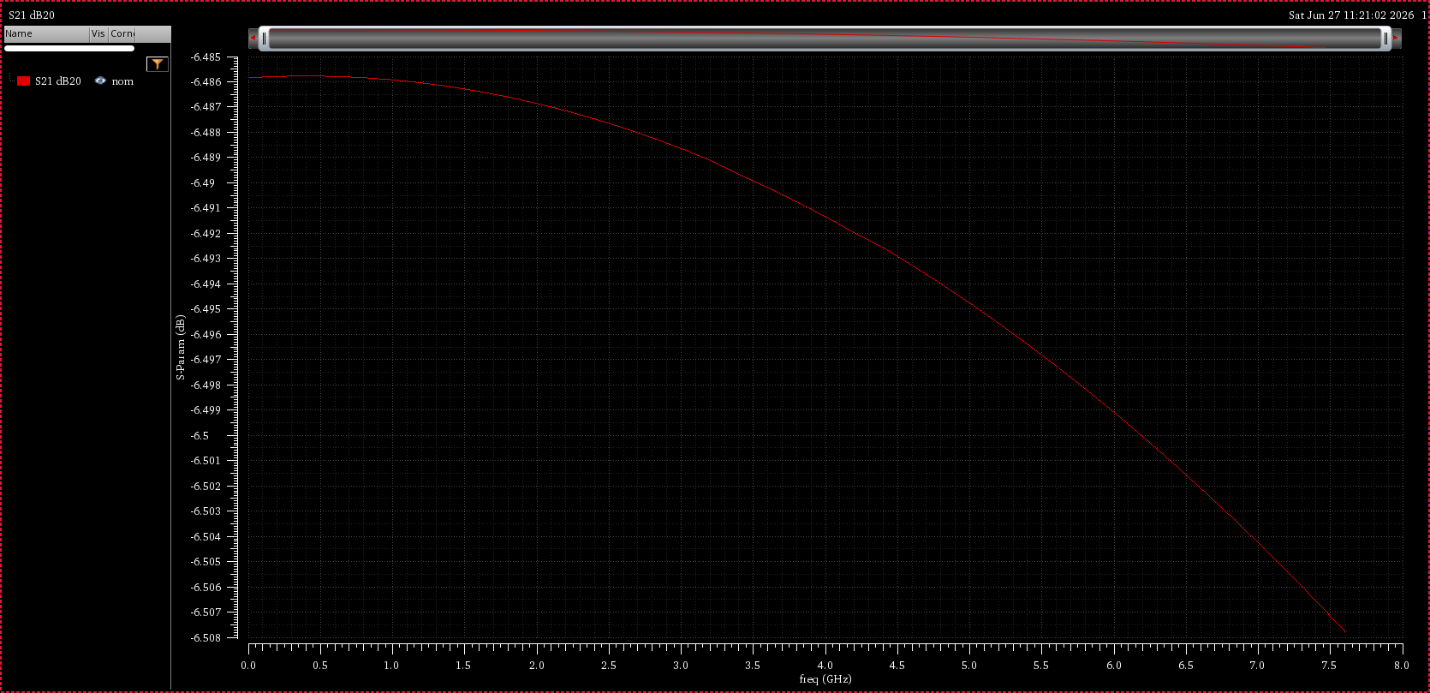
\includegraphics[width=\textwidth]{thesis_chapter_latex/figures/fig_lobuffer_mixer_gain_typical.png}
    \caption{Mixer conversion gain, typical case}
    \label{fig:lobuffer_mixer_gain_typical}
\end{figure}

\begin{figure}[htbp]
    \centering
    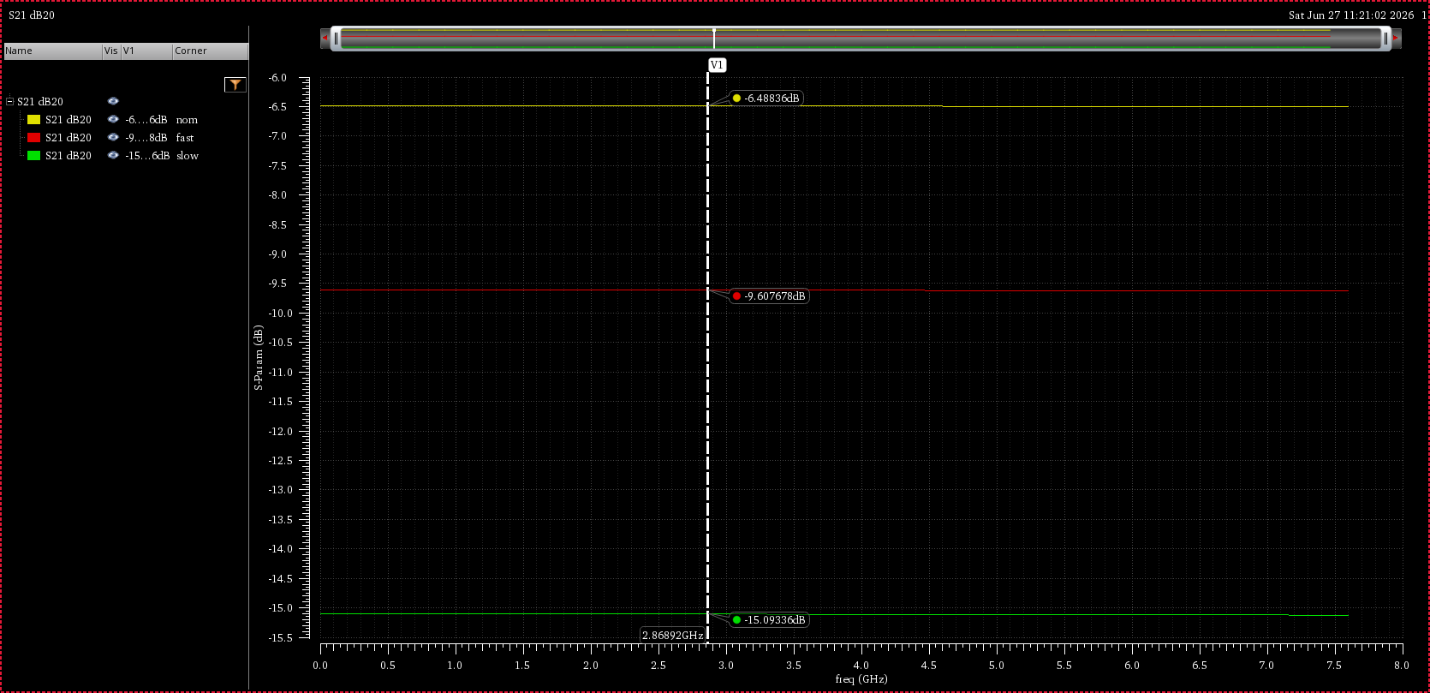
\includegraphics[width=\textwidth]{thesis_chapter_latex/figures/fig_lobuffer_mixer_gain_corners.png}
    \caption{Mixer conversion gain across corners}
    \label{fig:lobuffer_mixer_gain_corners}
\end{figure}

\textbf{Conversion Gain and Corner Deviation} --- The mixer's conversion gain satisfies the design target under nominal process and temperature conditions. However, the gain drops severely across the process corners, particularly at the slow-hot extreme. This significant corner degradation creates a large gain deficit, meaning a substantial amount of additional gain must be budgeted and distributed among the neighboring active stages in the receiver lineup to maintain the overall system sensitivity.

\subsection{IIP3}

IIP3 failed after adding the saturation amplifier: the mixer design was already at the edge of 11~dBm, and with the addition of the saturation amplifier it fails, dropping below 4~dBm.
